%----------------------------------------------------------------------------------------
%	PACKAGES AND OTHER DOCUMENT CONFIGURATIONS
%----------------------------------------------------------------------------------------

\documentclass[paper=a4, fontsize=11pt]{scrartcl} % A4 paper and 11pt font size

% ---- Entrada y salida de texto -----

\usepackage[T1]{fontenc} % Use 8-bit encoding that has 256 glyphs
\usepackage[utf8]{inputenc}
%\usepackage{fourier} % Use the Adobe Utopia font for the document - comment this line to return to the LaTeX default

% ---- Idioma --------

\usepackage[spanish, es-tabla]{babel} % Selecciona el español para palabras introducidas automáticamente, p.ej. "septiembre" en la fecha y especifica que se use la palabra Tabla en vez de Cuadro

% ---- Otros paquetes ----
\usepackage{csquotes} %Para permitir el uso de comillas Quotes https://tex.stackexchange.com/questions/36812/isnt-there-any-other-way-of-doing-double-quotes-in-latex-besides
\usepackage[hyphens]{url} % ,href} %para incluir URLs e hipervínculos dentro del texto (aunque hay que instalar href)
\usepackage{hyperref}
\usepackage{color}
\usepackage{graphics,graphicx, floatrow} %para incluir imágenes y notas en las imágenes
\usepackage{graphics,graphicx, float} %para incluir imágenes y colocarlas

\graphicspath {{./img/}}

\usepackage{listings}  %para introducir comandos

\lstdefinestyle{mybash}
{basicstyle=\ttfamily,
  showstringspaces=false,
  commentstyle=\color{red},
  keywordstyle=\color{blue},
  language=bash,
  alsoletter=/,
  basicstyle=\footnotesize,
  numbers=left,
  stepnumber=1,
  showstringspaces=false,
  tabsize=1,
  breaklines=true,
  breakatwhitespace=false,
}
\lstdefinestyle{mysql}
{basicstyle=\ttfamily,
  showstringspaces=false,
  commentstyle=\color{red},
  keywordstyle=\color{blue},
  language=sql,
  basicstyle=\footnotesize,
  numbers=left,
  stepnumber=1,
  showstringspaces=false,
  tabsize=1,
  breaklines=true,
  breakatwhitespace=false,
}


% Para hacer tablas comlejas
%\usepackage{multirow}
%\usepackage{threeparttable}

%\usepackage{sectsty} % Allows customizing section commands
%\allsectionsfont{\centering \normalfont\scshape} % Make all sections centered, the default font and small caps

\usepackage{fancyhdr} % Custom headers and footers
\pagestyle{fancyplain} % Makes all pages in the document conform to the custom headers and footers
\fancyhead{} % No page header - if you want one, create it in the same way as the footers below
\fancyfoot[L]{} % Empty left footer
\fancyfoot[C]{} % Empty center footer
\fancyfoot[R]{\thepage} % Page numbering for right footer
\renewcommand{\headrulewidth}{0pt} % Remove header underlines
\renewcommand{\footrulewidth}{0pt} % Remove footer underlines
\setlength{\headheight}{13.6pt} % Customize the height of the header

\setlength\parindent{0pt} % Removes all indentation from paragraphs - comment this line for an assignment with lots of text

\newcommand{\horrule}[1]{\rule{\linewidth}{#1}} % Create horizontal rule command with 1 argument of height


%----------------------------------------------------------------------------------------
%	TÍTULO Y DATOS DEL ALUMNO
%----------------------------------------------------------------------------------------
\graphicspath{ {img/} }

\title{
\normalfont \normalsize

\includegraphics[width=6cm,height=6cm]{logo}\\
\textsc{\textbf{Bootcamp Especialidad GNU/Linux (2023)}} \\ [25pt] % Your university, school and/or department name(s)
\horrule{0.5pt} \\[0.4cm] % Thin top horizontal rule
\huge Lab 10 - Servidor de Correo \\ % The assignment title
\horrule{2pt} \\[0.5cm] % Thick bottom horizontal rule
}

%https://es.overleaf.com/learn/latex/Inserting_Images
%Ruta relativa de   imagenes

\author{Pedro Antonio Mayorgas Parejo} % Nombre y apellidos

\date{\normalsize\today} % Incluye la fecha actual

%----------------------------------------------------------------------------------------
% DOCUMENTO
%----------------------------------------------------------------------------------------

\begin{document}

\maketitle % Muestra el Título

\newpage %inserta un salto de página

\tableofcontents % para generar el índice de contenidos

\newpage

%----------------------------------------------------------------------------------------
%	Cuestión 1
%----------------------------------------------------------------------------------------

\section{Topología de red}
Se ha seguido una topología de red que nos ha permitido conectar por capa 2 los dispositivos y que estos puedan acceder a servicios de DNS compartidos sin tener que modificar nada más.

\begin{turn}{90}   
    \centering
    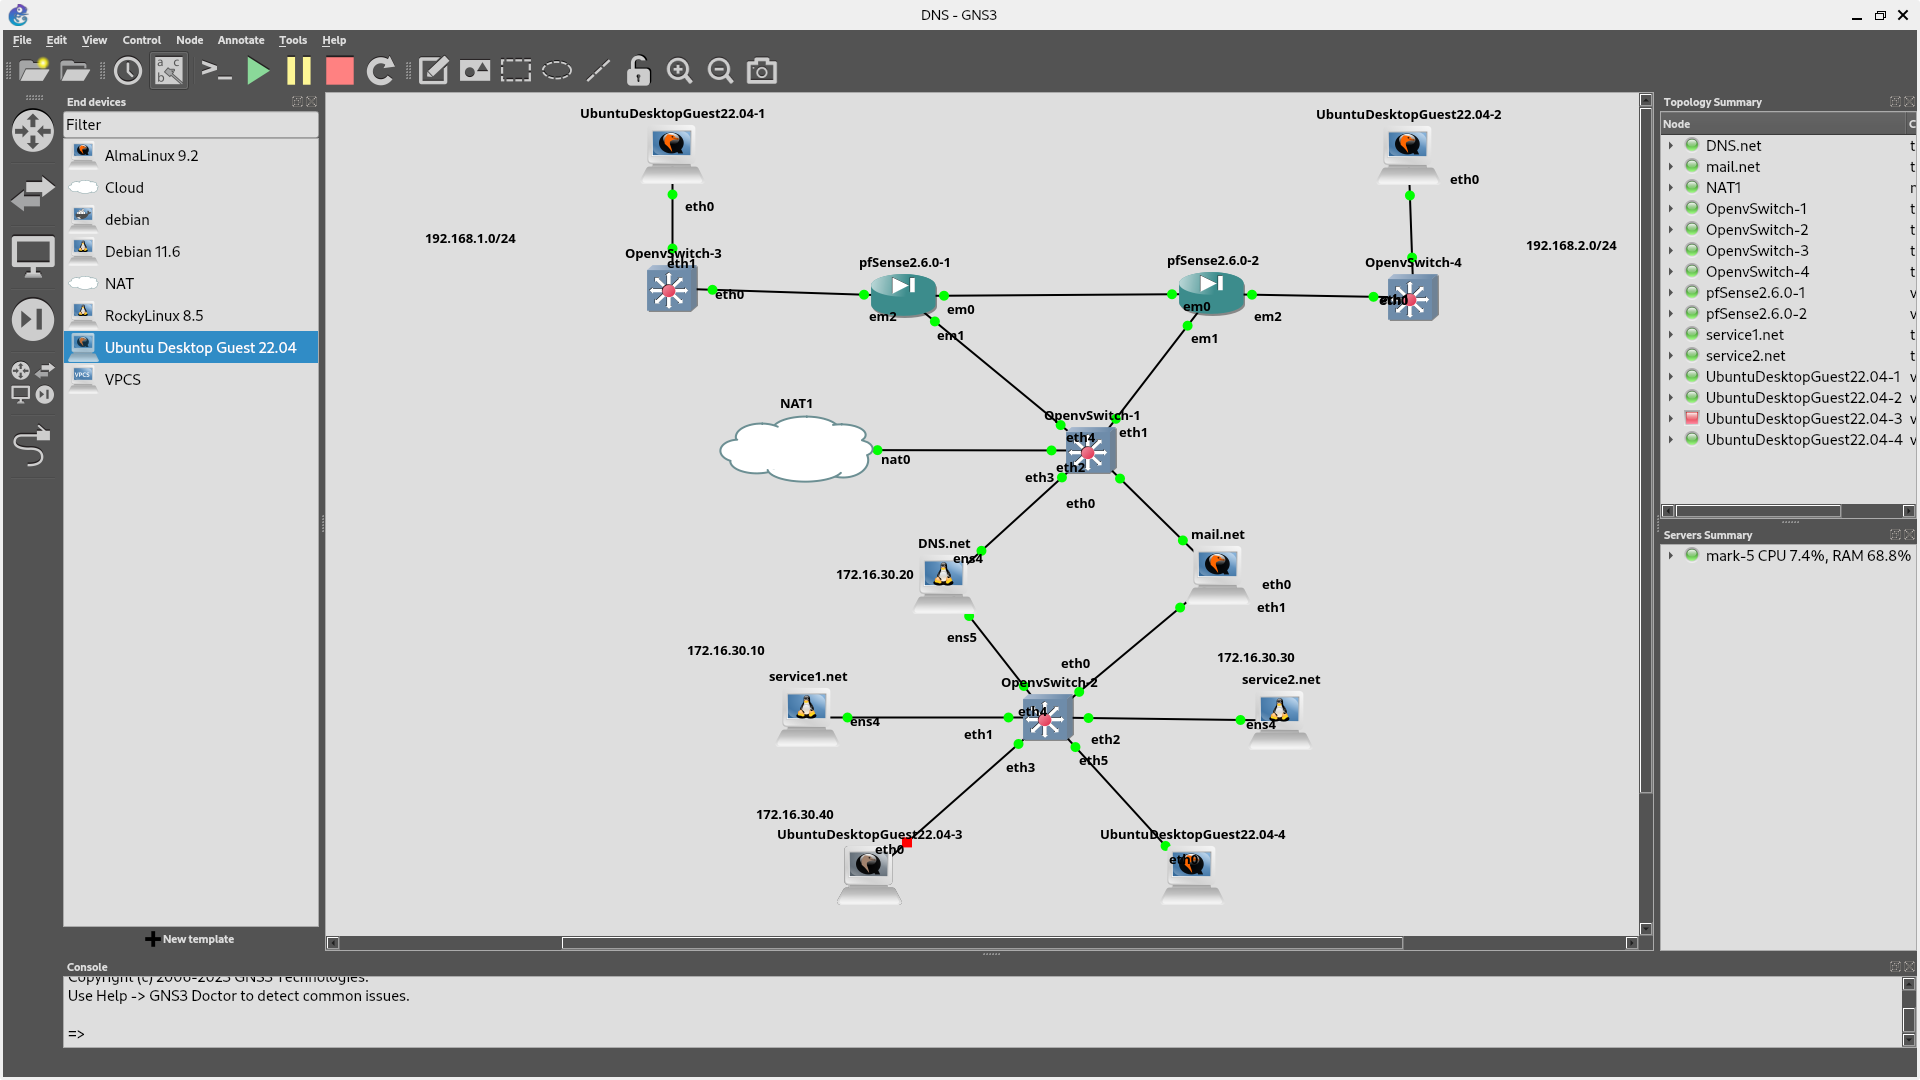
\includegraphics[scale=0.25]{30}
\end{turn}

\newpage
\section{Preparación de DNS}

En primer lugar, tenemos que preparar el servicio DNS, para poder utilizar el registro MX utilizado para los servicios de correo asociados. Así como podemos indicar la preferencia de los servidores de correo, porque podemos indicar más de uno. El valor más bajo de preferencia, es el que mayor prioridad queremos que tenga, por convención se usa el 10, 20, 30...

\begin{figure}[H]
	\centering
	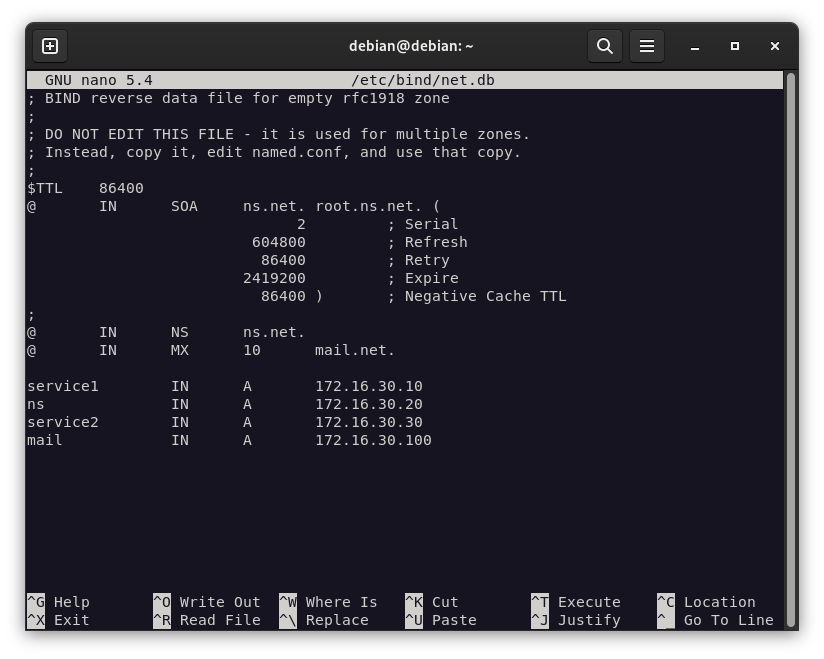
\includegraphics[scale=0.30]{00}
	\caption{Registros de DNS, de la zona.}
\end{figure}


Una vez que hayamos terminado de preparar los registros de la zona MX, también tenemos que indicar el registro A, para que la resolución de DNS, tenga una dirección IP a la que acudir. La siguiente captura son las pruebas, donde usamos el comando dig, para obtener un servidor de correo con el registro MX de la zona.

\begin{figure}[H]
	\centering
	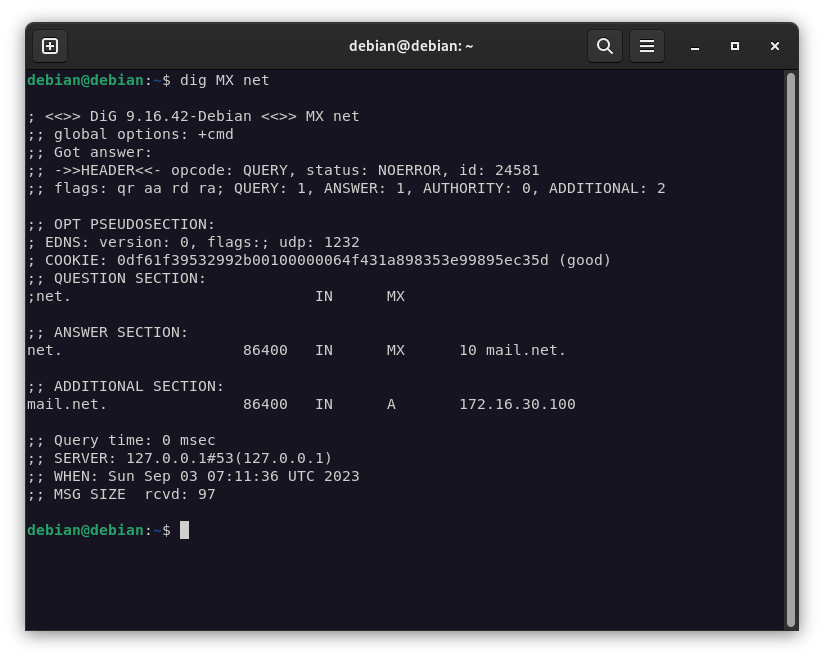
\includegraphics[scale=0.30]{01}
	\caption{Pruebas del servicio DNS.}
\end{figure}


Todos los comandos que han sido utilizados son:

\begin{lstlisting}[style=mybash]
sudo systemctl restart bind9.service
sudo systemctl status bind9.service
\end{lstlisting}

Una vez que se han reiniciado los servicios, debemos también comprobar que se hayan cargado las zonas de DNS correctamente, para ello con el último comando que se ha indicado anteriormente, se debe comproabr que aparezca un \textbf{all zones loaded}.

\section{Instalación de Postfix MTA}

Postfix es un MTA Mail Transfer Agent, que te permite el envío de correos electrónicos por el protocolo SMTP (Simple Mail Transfer Protocol). Es un MTA muy robusto que permite una amplia configuración.
\vspace{5mm}

Para la instalación de Postfix, hemos utilizado una distribución basada en Red Hat, para poder seguir un manual profesional de configuración del MTA. La mayoría de los cambios se han concrentrado en el fichero \textbf{main.cf}, dicho fichero se localiza en \textbf{/etc/postfix/main.cf}. En la documentación de Red Hat se indica que hay que concentrarse en la configuración inicial de los siguientes parámetros del fichero de configuración, para que pueda configurarse de manera básica el MTA.
\vspace{5mm}

Comando para instalar Postfix en las distribuciones Red Hat:

\begin{lstlisting}[style=mybash]
sudo dnf update
sudo dnf install postfix
\end{lstlisting}

\begin{figure}[H]
	\centering
	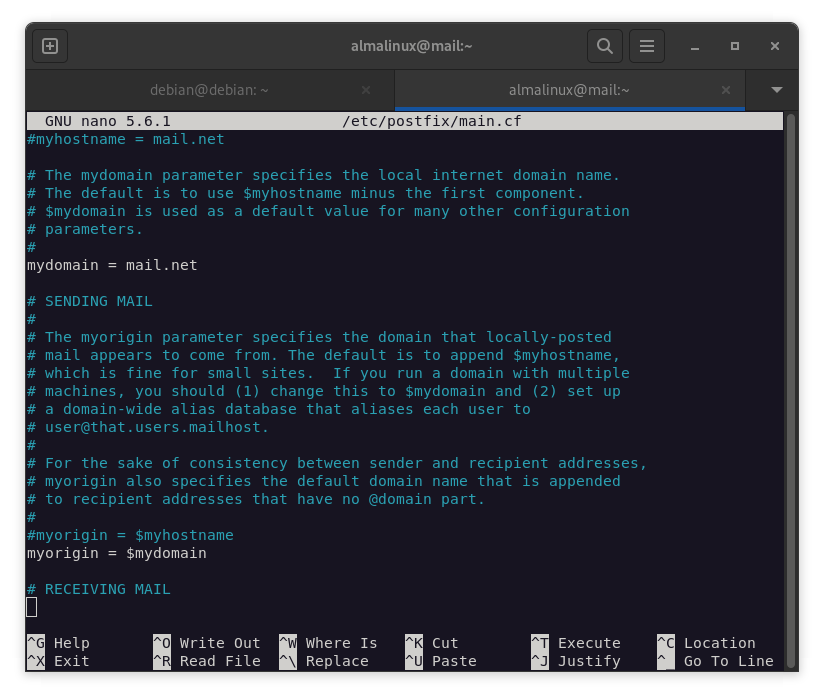
\includegraphics[scale=0.30]{02}
	\caption{Parámetros de main.cf - Configuración del dominio y origen.}
\end{figure}

En la captura anterior, se tiene que configurar el dominio local del servicio de correo. Puede ser mx.dominio.tld, o dominio.tld indistintamente. Luego el siguiente parámetro que hemos configurado, es el de origin, que es el parámetro utilizado para indicar el origen de mensajes enviados desde este MTA o sus usuarios.

\begin{figure}[H]
	\centering
	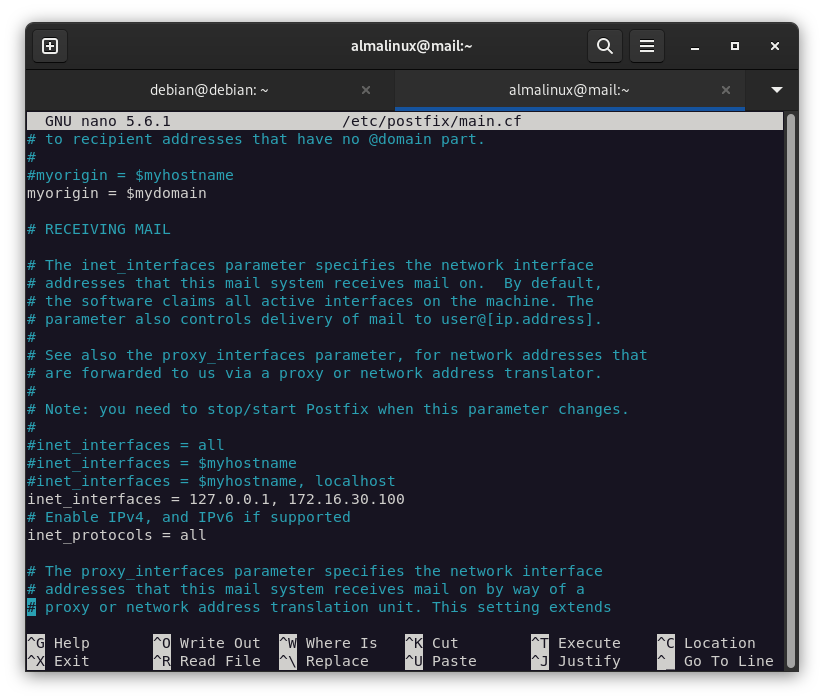
\includegraphics[scale=0.30]{03}
	\caption{Parámetros de main.cf - Configuración de las interfaces de recepción de email.}
\end{figure}

Ahora tenemos que configurar las interfaces por las que Postfix recibe los correos, en el manual de administración se puede indicar un parámetro especial \textbf{all}, pero esto implica que se ponga el correo en escucha en todas las interfaces de red indistintamente,lo cual no suele ser bueno. En su lugar, he configurado dos interfaces, en la cual una es la dirección IP externa y otra que debería de estár de manera obligatoria que es la dirección de loopback o localhost.

\begin{figure}[H]
	\centering
	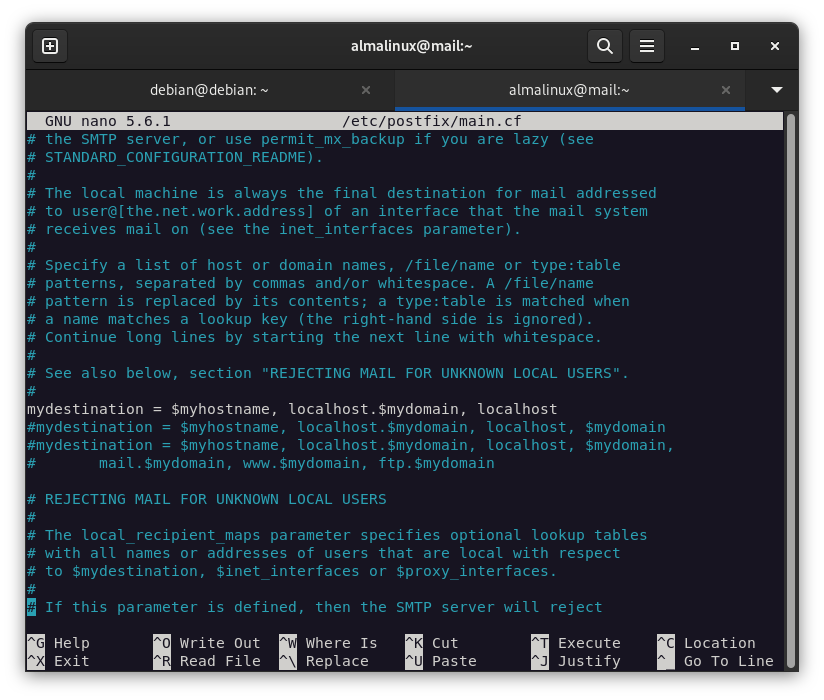
\includegraphics[scale=0.30]{04}
	\caption{Parámetros de main.cf - Configuración de destinatarios en el MTA.}
\end{figure}

Luego tenemos que configurar el parámetro de \textbf{mydestination}, que consiste en cómo acepta de manera interna el MTA que es un destinatario que se envía de manera local, en vez de hacer reenvío. La configuración indicada en el manual de postfix es el caso 1, donde es el caso por defecto.
\vspace{5mm}

Una vez terminada la configuración anterior, debemos ejecutar el comando siguiente para comprobar si la configuración del main.cf de Postfix contiene algún error.

\begin{lstlisting}[style=mybash]
sudo postfix check
\end{lstlisting}

Luego de configurar Postfix, debemos activar y habilitar el servicio con el siguiente comando:

\begin{lstlisting}[style=mybash]
sudo systemctl enable --now postfix.service
# Verify
sudo systemctl status postfix
\end{lstlisting}

Luego tenemos que probar el servicio de correo, para ello instalar la siguiente utilidad que nos permite usar el MTA para enviar correos a los usuarios locales, claro que tenemos que crear previamente al usuario para poder enviarle el mail, así como para poder autenticarnos y leer su correo final en /var/log/maillog o en 
\begin{lstlisting}[style=mybash]
sudo dnf install sendmail
nano mail.txt
sendmail pedro@mail.net < mail.txt
\end{lstlisting}

\begin{figure}[H]
	\centering
	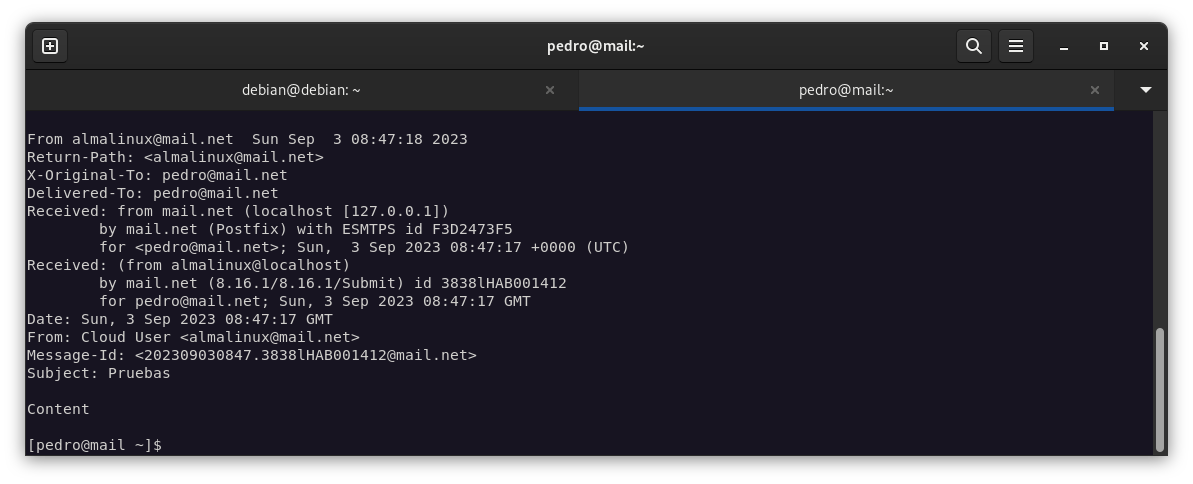
\includegraphics[scale=0.30]{05}
	\caption{Recepción del correo electrónico.}
\end{figure}

Para poder ver los correos, vamos a \textbf{/var/log/mail/\$USER}. 

\begin{figure}[H]
	\centering
	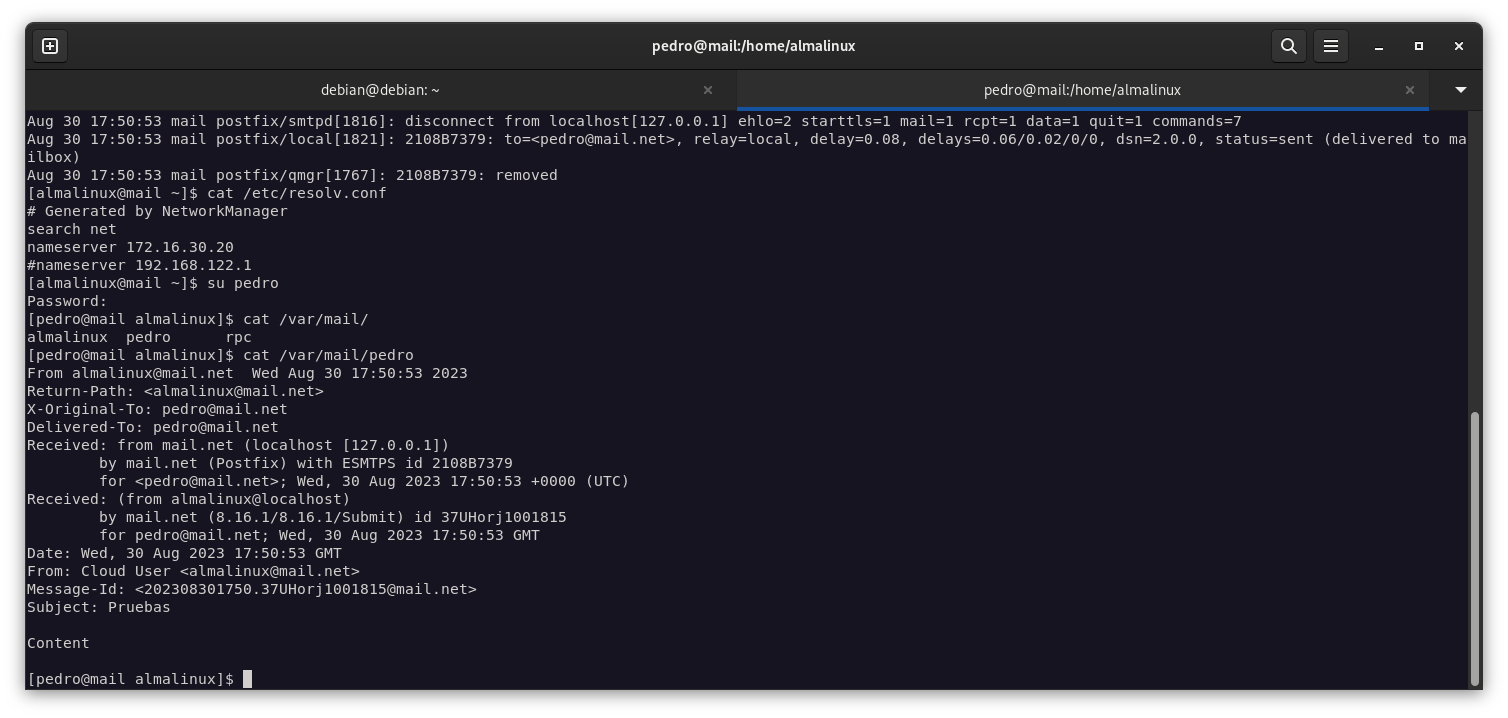
\includegraphics[scale=0.30]{07}
	\caption{Correos en /var/log/mail/.}
\end{figure}

Por último tenemos que configurar el \textbf{home\_mailbox}, para que podamos tenerlo en el \$HOME del usuario, sobre todo a la hora de que Dovecot pueda leer los mensajes para utilizarlos con los protocolos clientes de IMAP o POP3.

\begin{figure}[H]
	\centering
	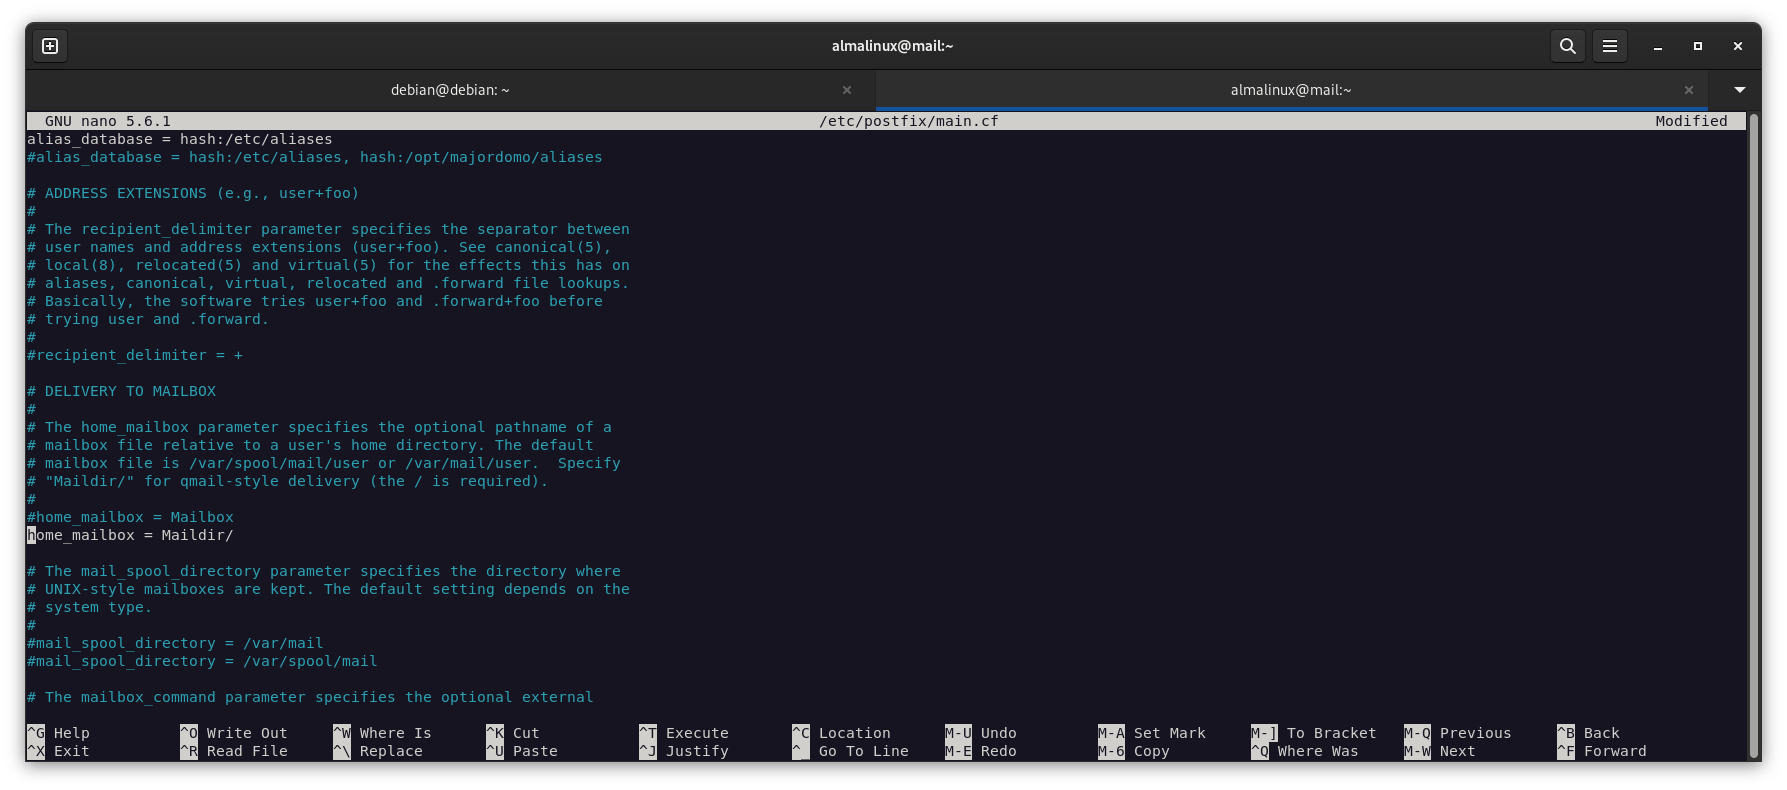
\includegraphics[scale=0.25]{06}
	\caption{Configuración del home de los correos.}
\end{figure}

Ahora inicializamos el servicio y comprobamos si hay errores.
\begin{lstlisting}[style=mybash]
sudo postfix check
# Habilitamos el arranque del servicio
sudo systemctl enable postfix.service
sudo systemctl start postfix.service
# Comprobamos si hay errores
sudo journalctl -xeu dovecot.service
\end{lstlisting}


\subsection{TLS en Postfix}

Ahora tenemos que configurar TLS en el Postfix para hacer el envío y recepción seguros con TLS. Primero tenemos que generar una clave privada que nos permita el cifrado asimétrico clásico de RSA que se usa en TLS, luego tenemos que generar a partir de esa clave privada el certificado público de tipo x509 que el servidor provee a los clientes.

\begin{lstlisting}[style=mybash]
# PRIVATE KEY GEN
sudo openssl genrsa -out /etc/pki/mail.key.pem 2048
# PUBLIC AND CERT x509 GEN
sudo openssl req -key /etc/pki/mail.key.pem -new -x509 -days 365 -out /etc/pki/mail.cert.pem
\end{lstlisting}

\begin{figure}[H]
	\centering
	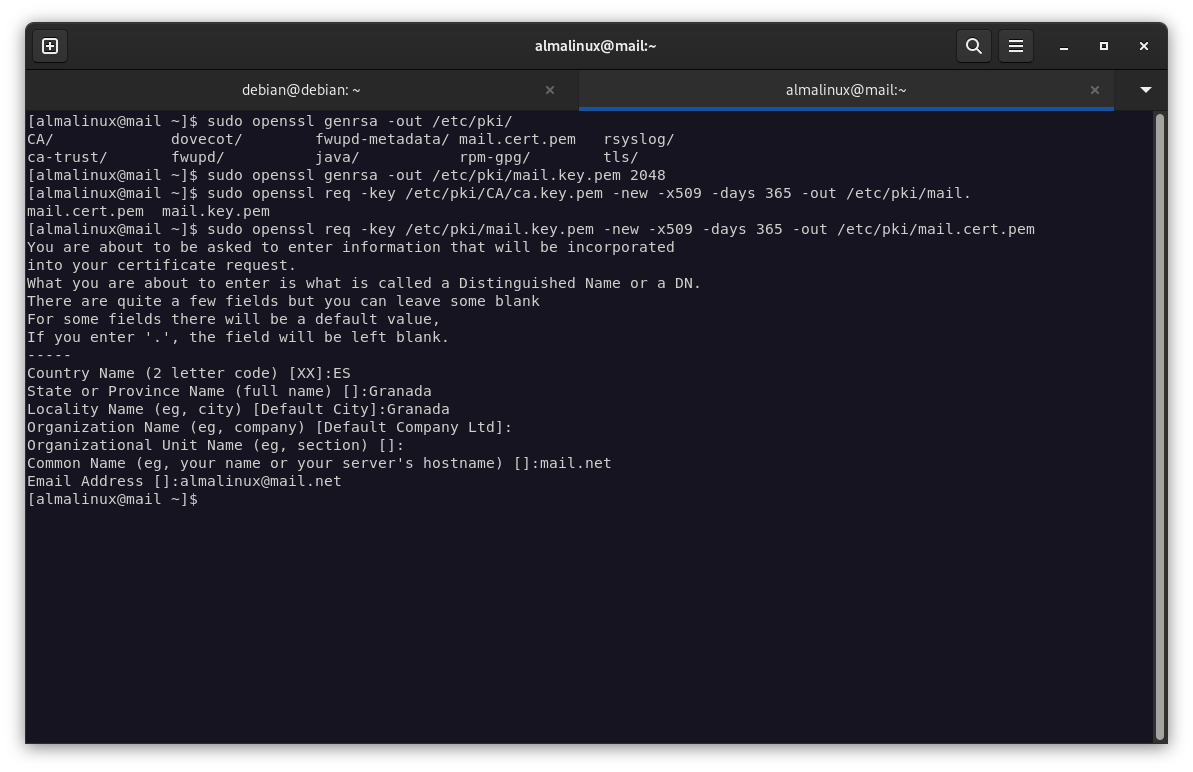
\includegraphics[scale=0.30]{08}
	\caption{Generación del certificado SSL para mail.net}
\end{figure}

Ahora tenemos que configurar el servidor Postfix, para que pueda utilizar correctamente el certificaodo, por defecto en las últimas actualizaciones al parecer usa un certificado flojo, para poder ofrecer conexiones un poco más seguras que en texto plano. Para configurar dicho certificado debemos ir a \textbf{/etc/postfix/main.cf}. Tenemos que modificar los siguientes parámetros. 

\textbf{Nota:} Los parámetros los tenemos que indicar dos veces, debido a que uno es para la recepción y otro es para el envío. Entonces si uno de ellos se omite, ocurrirá que se envíen los datos en texto plano.

\begin{figure}[H]
	\centering
	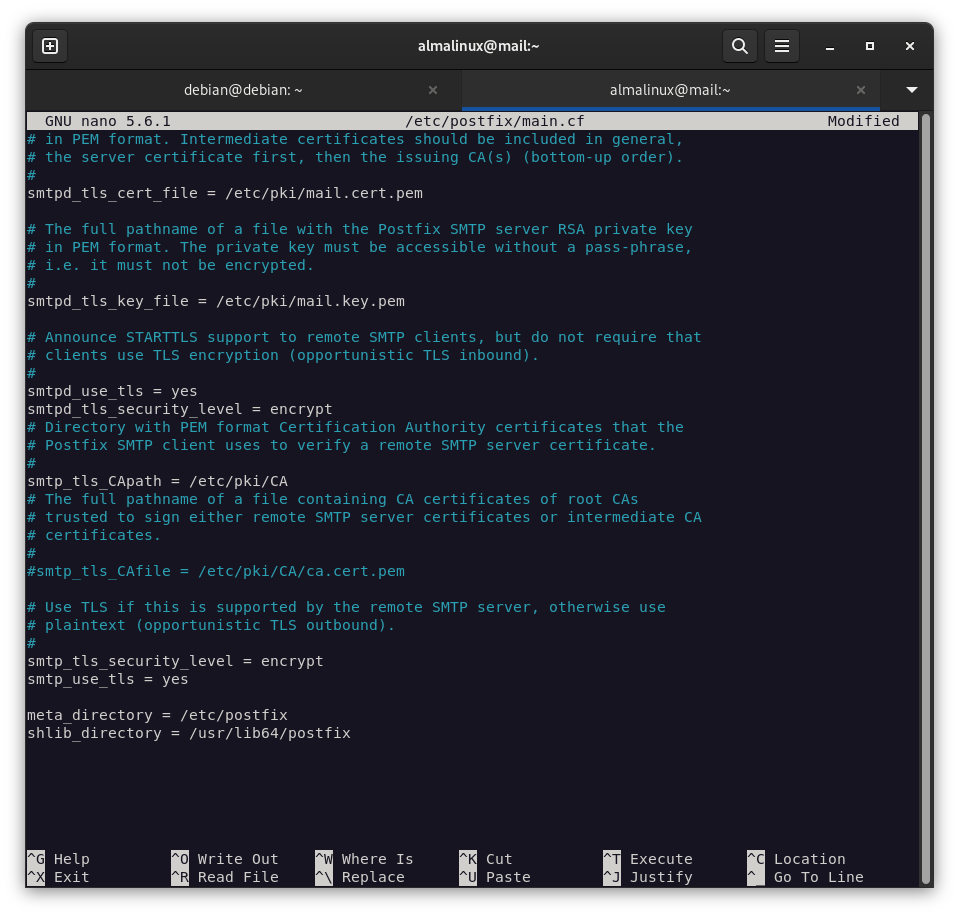
\includegraphics[scale=0.30]{09}
	\caption{Configuración utilizada para STARTTLS}
\end{figure}

Ahora inicializamos el servicio y comprobamos si hay errores.

\begin{lstlisting}[style=mybash]
# Comprobador de si hay fallos en los ficheros de configuracion
sudo postfix check
sudo systemctl restart postfix.service
# Comprobamos si hay errores adicionales
sudo journalctl -xeu postfix.service
\end{lstlisting}


Finalmente para probar el STARTTLS, podemos instalar netcat y interaccionar con el servidor para que nos pase los parámetros. Dentro de ellos, debe poner STARTTLS.

\begin{lstlisting}[style=mybash]
nc mail.net 25
ehlo test
\end{lstlisting}

\begin{figure}[H]
	\centering
	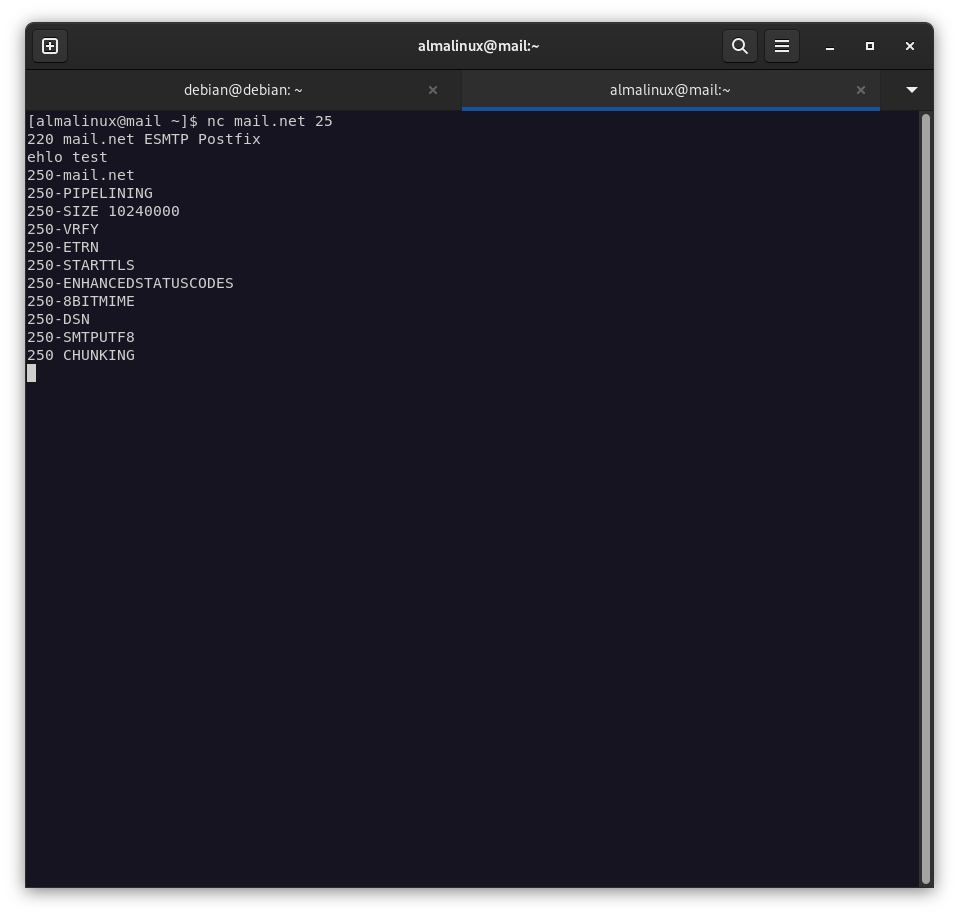
\includegraphics[scale=0.30]{10}
	\caption{Pruebas de STARTTLS}
\end{figure}

\newpage 
\section{Instalación y configuración de Dovecot}

Ahora tenemos que realizar la instalación de Dovecot con el siguiente comando:

\begin{lstlisting}[style=mybash]
sudo dnf install dovecot
\end{lstlisting}

Los ficheros de configuración de Dovecot, se encuentran en \textbf{/etc/dovecot/dovecot.conf}, lo primero que debemos configurar son los protocolos que va a soportar. Así como las direcciones IP que debe escuchar.

\begin{figure}[H]
	\centering
	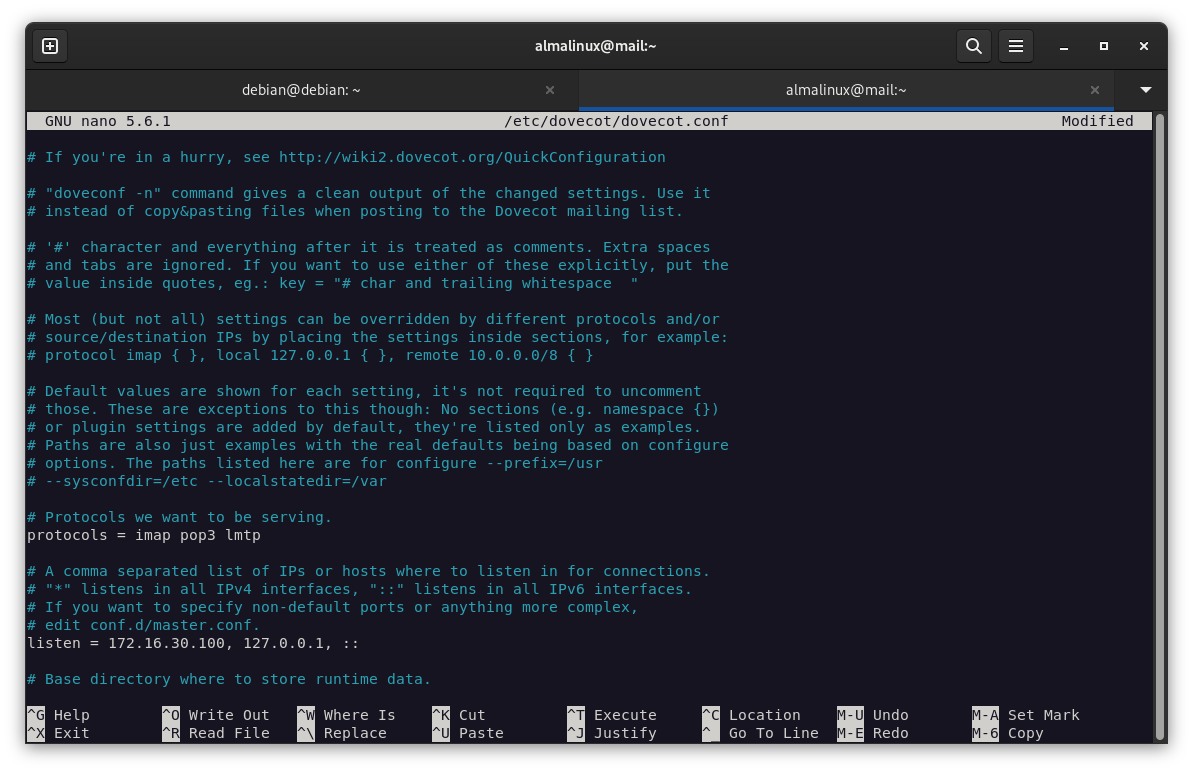
\includegraphics[scale=0.30]{11}
	\caption{Configuración de protocolos de Dovecot}
\end{figure}

Luego debemos indicar el mecanismo de autenticación de login adicional al de plain. Todo eso está localizado en \textbf{/etc/dovecot/10-auth.conf}.

\begin{figure}[H]
	\centering
	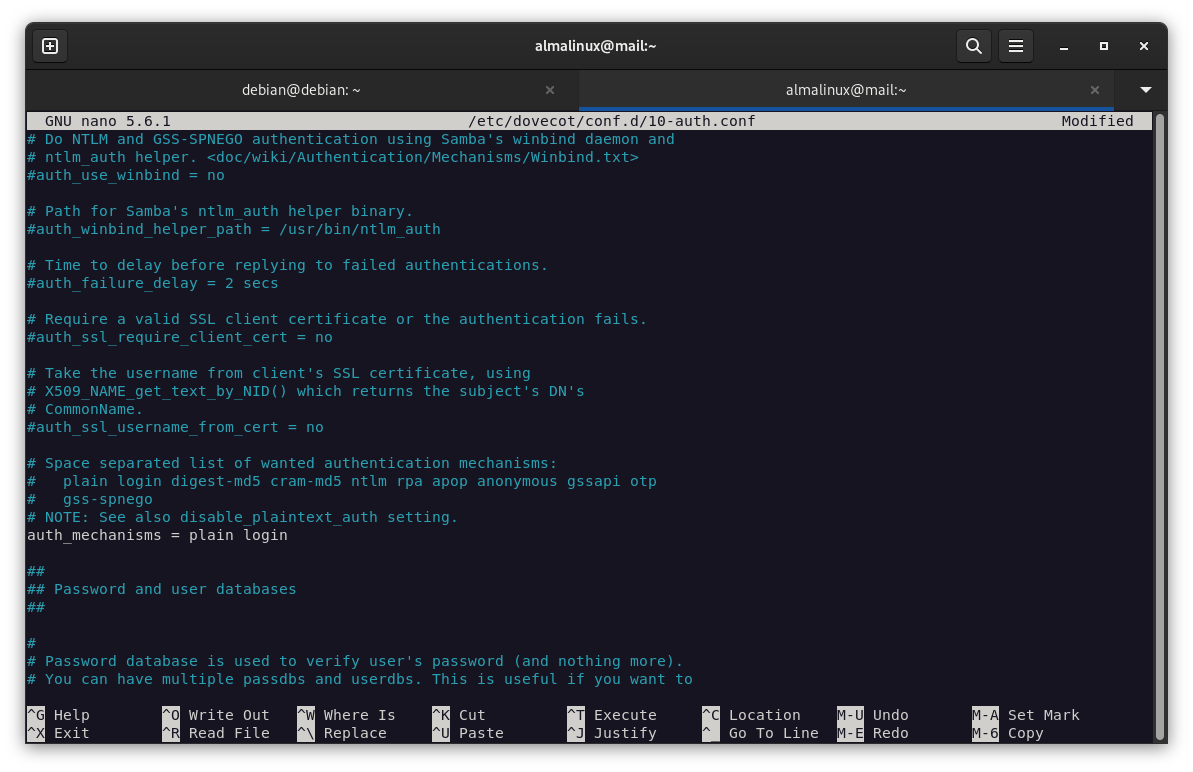
\includegraphics[scale=0.30]{12}
	\caption{Configuración de autenticación de Dovecot}
\end{figure}

Luego debemos configurar el directorio de la bandeja de entrada y salida del usuario. Puede estar ubicado en el \textbf{\$HOME} o en \textbf{/var/mail/\$USER}.

\begin{figure}[H]
	\centering
	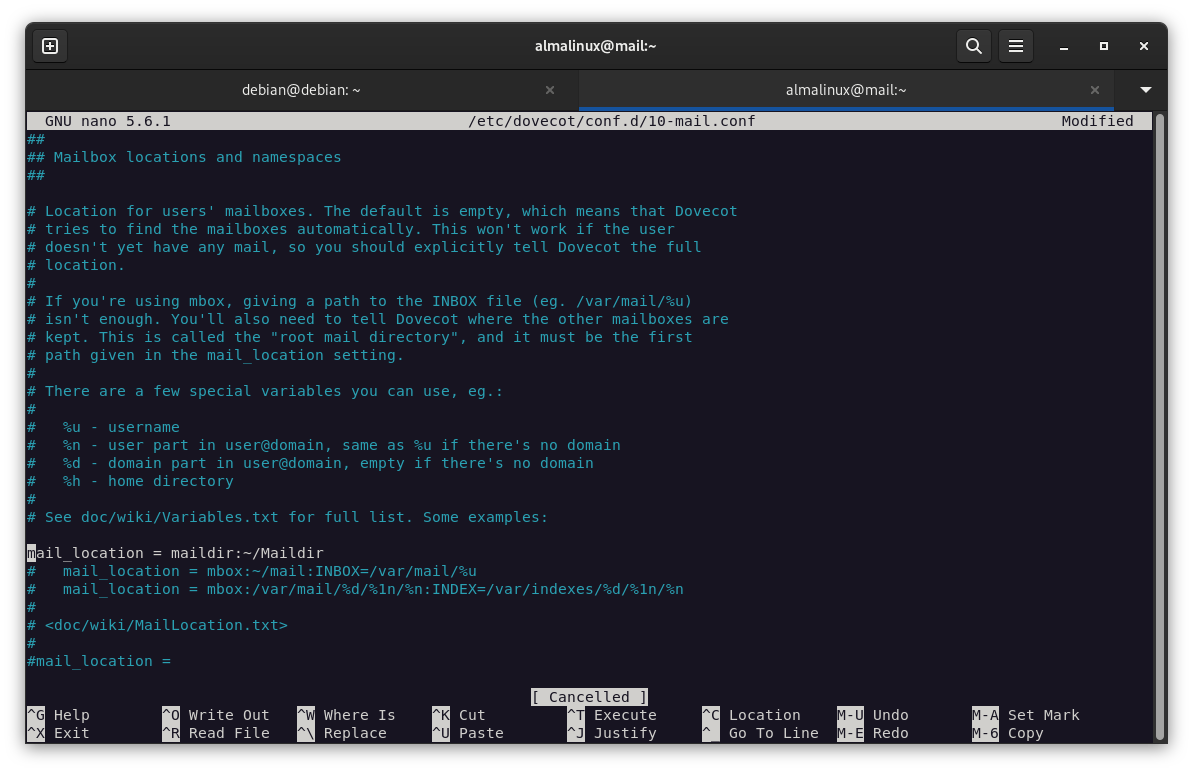
\includegraphics[scale=0.30]{13}
	\caption{Directorio del mail}
\end{figure}

Ahora queremos configurar que Postfix, pueda usar Dovecot para la recepción de los mensajes y que este los cataloge en los subdirectorios correspondientes. Para ello debemos contactarlos con el Socket correspondiente. El protocolo que usan es lmtp entre ellos, se ha configurado anteriormente

\begin{figure}[H]
	\centering
	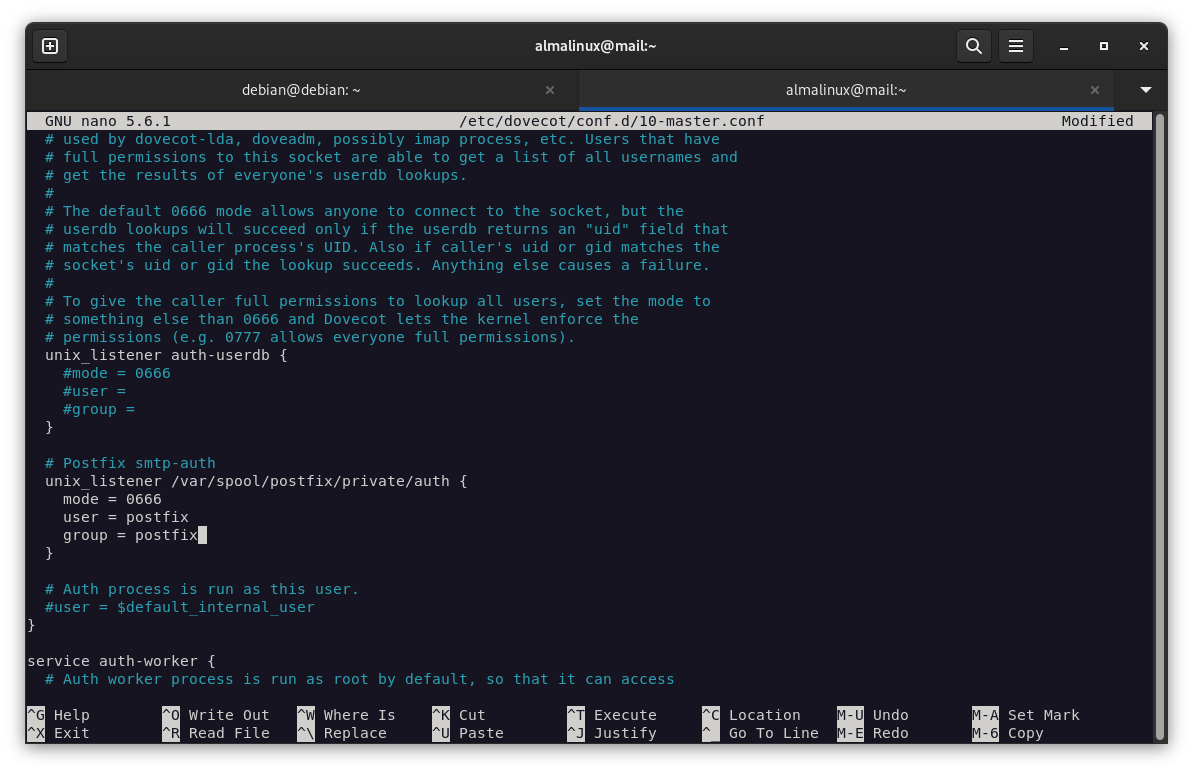
\includegraphics[scale=0.30]{14}
	\caption{Configuración del Socket}
\end{figure}

Por último configuramos los certificados compartidos con Postfix, para el uso de conexiones seguras en la ruta \textbf{/etc/dovecot/10-ssl.conf}

\begin{figure}[H]
	\centering
	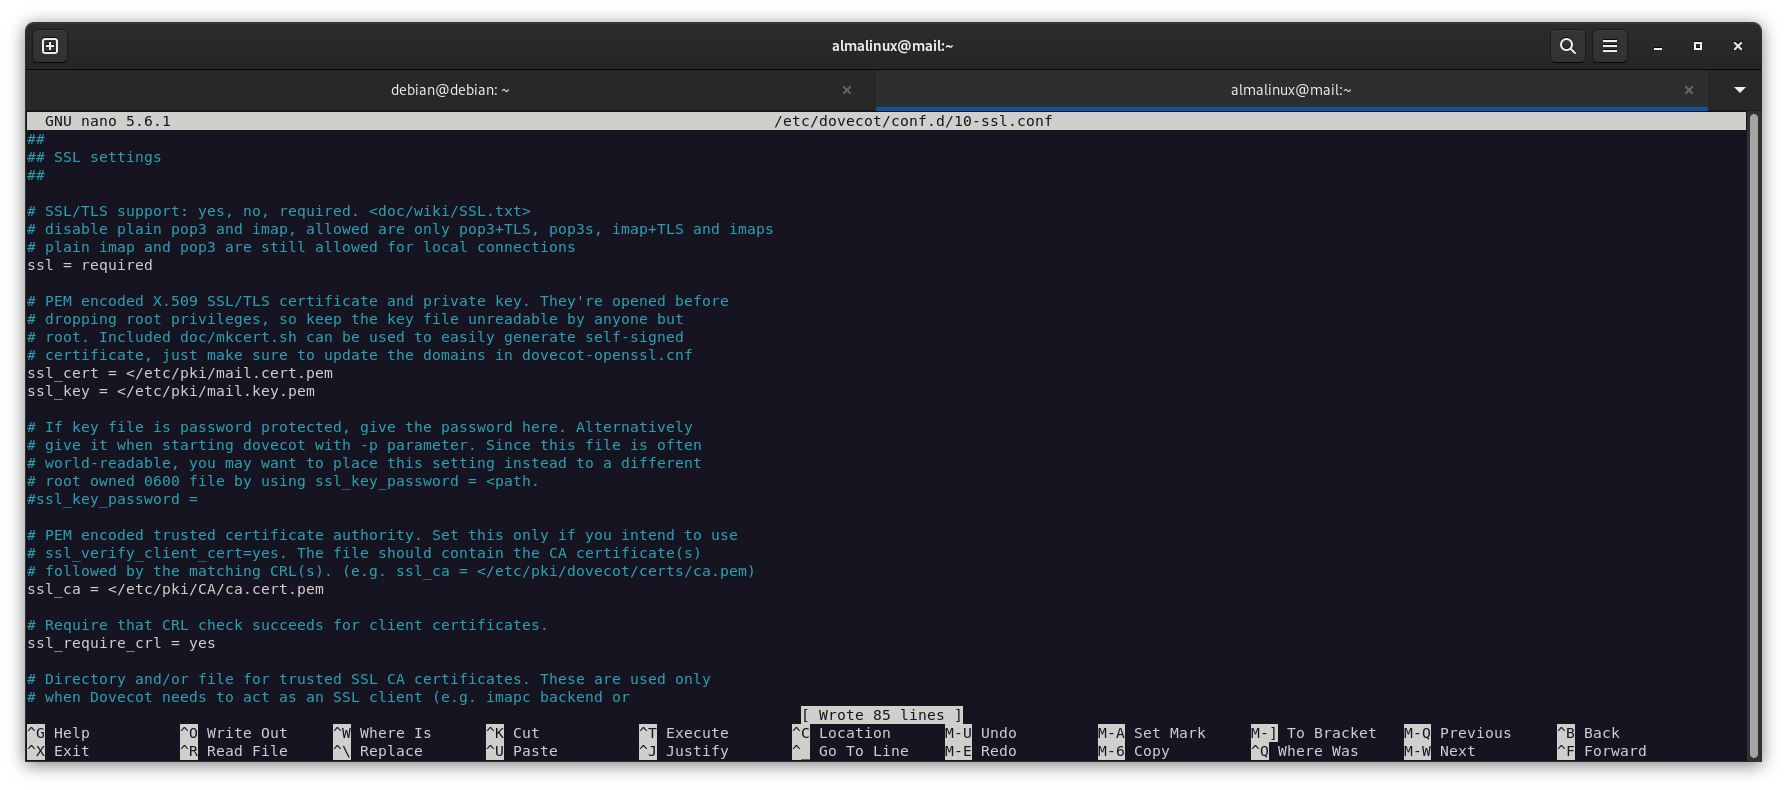
\includegraphics[scale=0.25]{26}
	\caption{Configuración SSL}
\end{figure}

Ahora inicializamos el servicio y comprobamos si hay errores.
\begin{lstlisting}[style=mybash]
sudo systemctl enable dovecot.service
sudo systemctl start dovecot.service
# Comprobamos si hay errores
sudo journalctl -xeu dovecot.service
\end{lstlisting}

Ahora nos vamos a un cliente de correo (Thunderbird) y usamos IMAP siguiendo los siguientes pasos.

\begin{figure}[H]
	\centering
	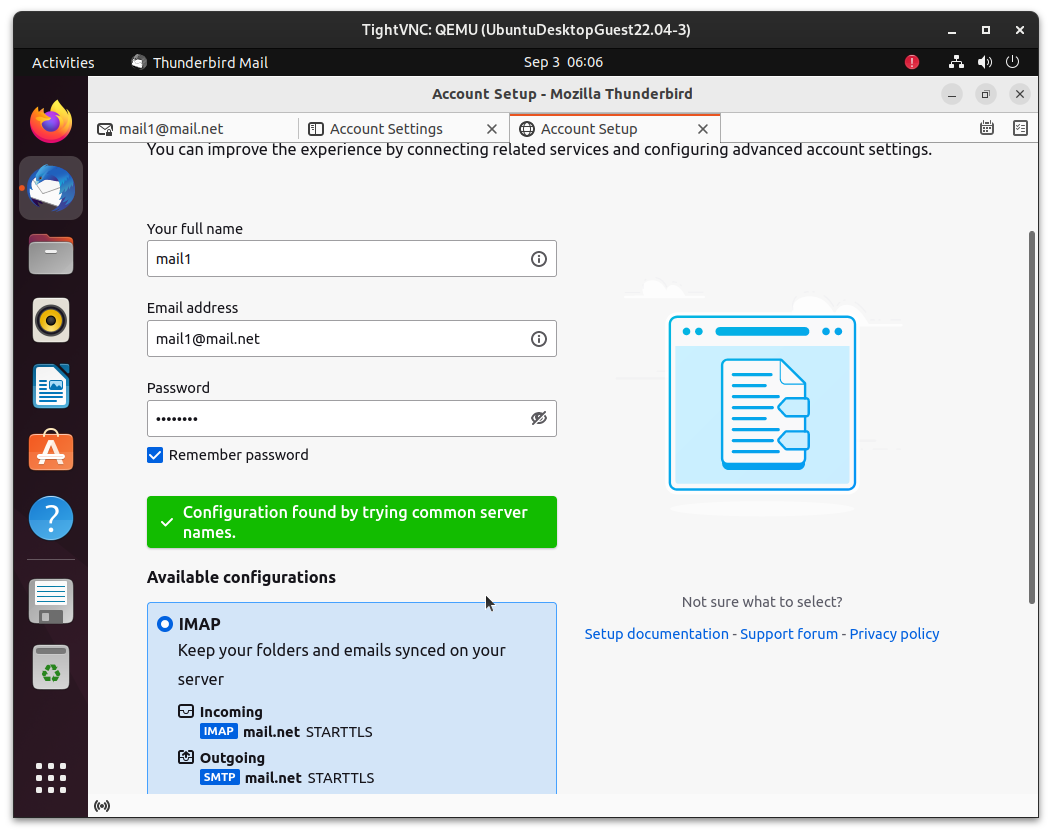
\includegraphics[scale=0.30]{15}
	\caption{Introduciendo las credenciales}
\end{figure}

\begin{figure}[H]
	\centering
	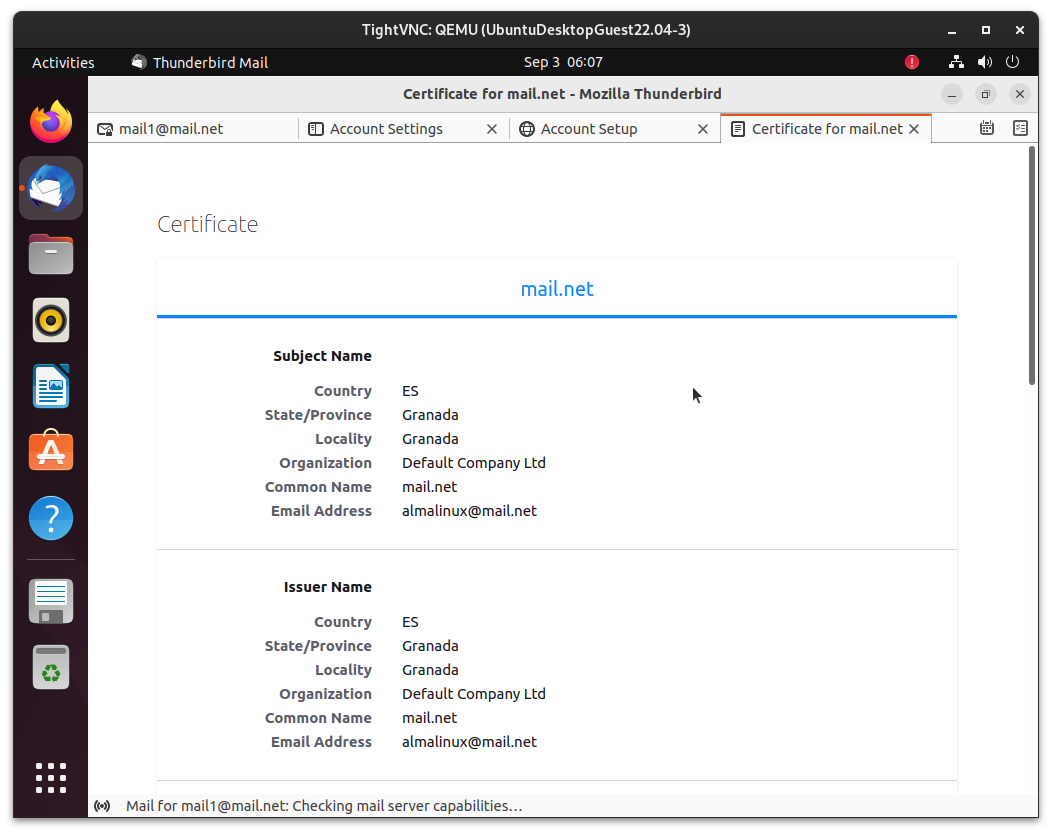
\includegraphics[scale=0.30]{16}
	\caption{Verificando el certificado.}
\end{figure}

\begin{figure}[H]
	\centering
	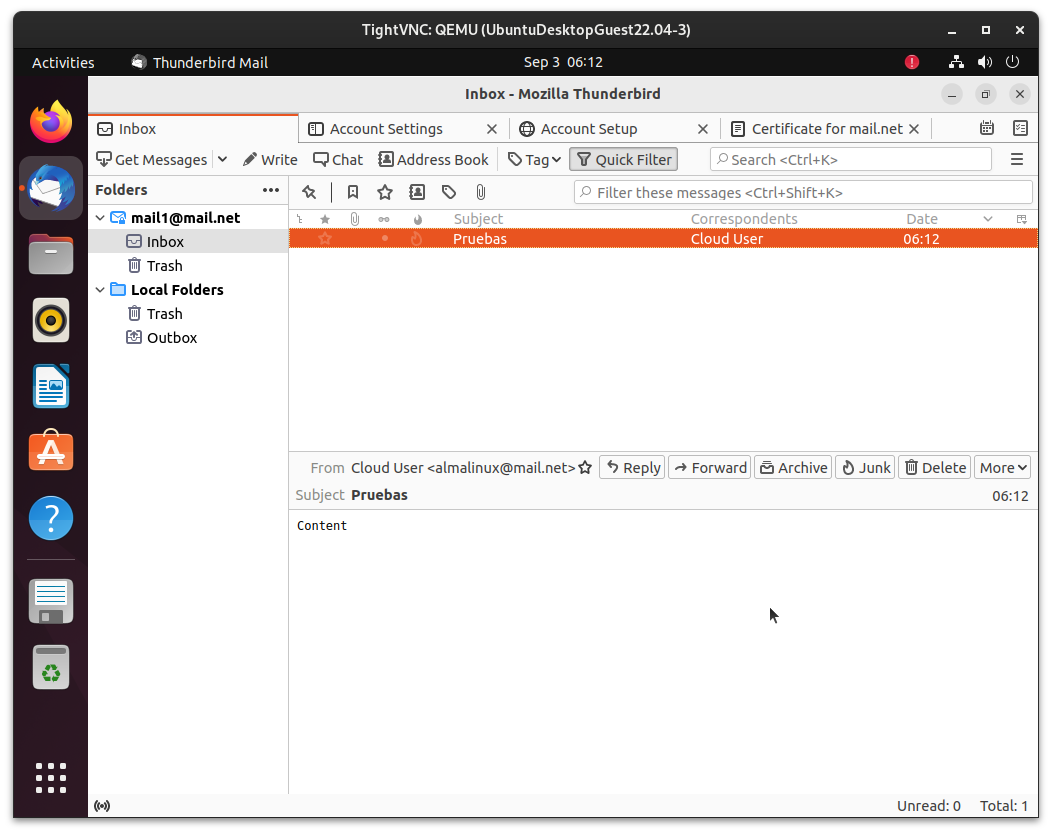
\includegraphics[scale=0.30]{17}
	\caption{Recepción de mensajes.}
\end{figure}

\begin{figure}[H]
	\centering
	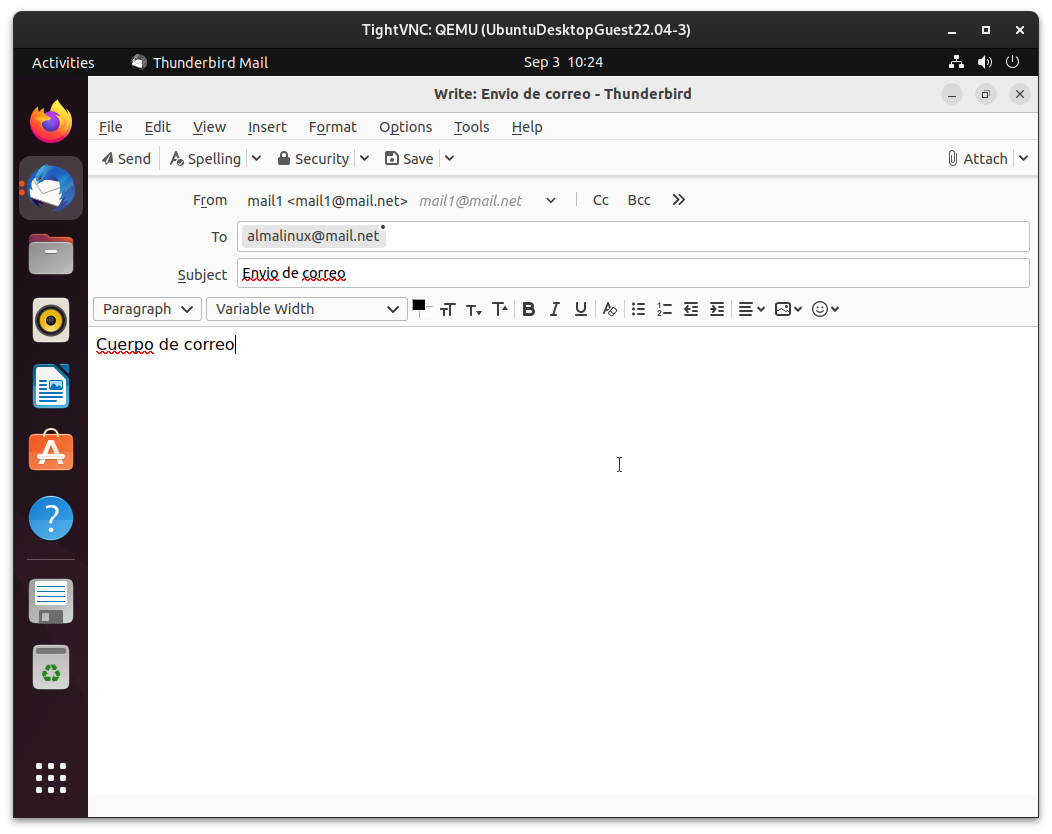
\includegraphics[scale=0.30]{18}
	\caption{Envío de mensajes.}
\end{figure}

\begin{figure}[H]
	\centering
	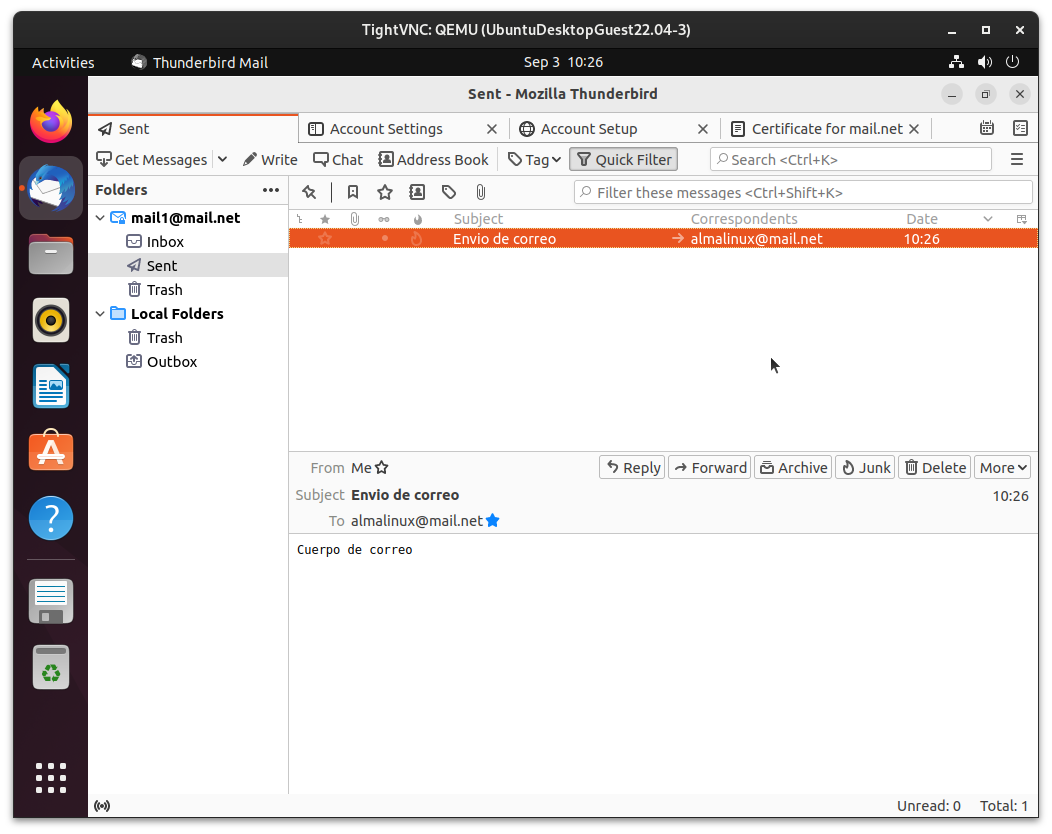
\includegraphics[scale=0.30]{19}
	\caption{Envío de mensajes - parte 2.}
\end{figure}

\begin{figure}[H]
	\centering
	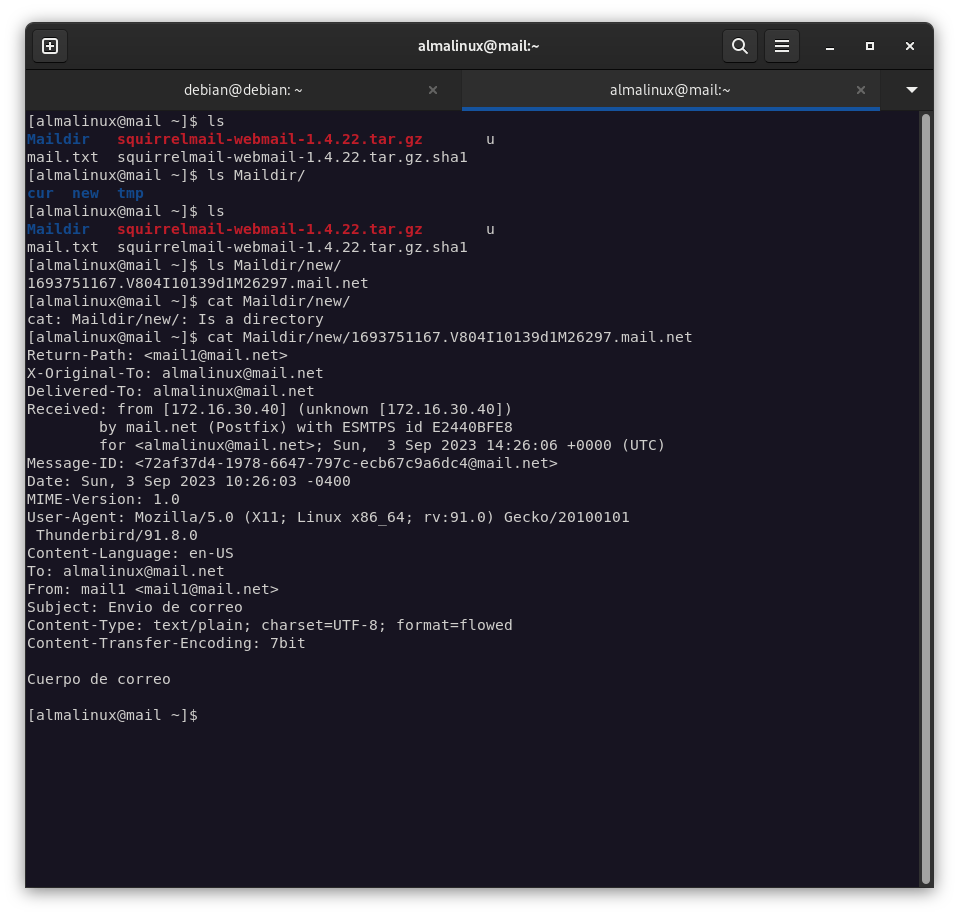
\includegraphics[scale=0.30]{20}
	\caption{Envío de mensajes - parte 3.}
\end{figure}



\newpage
\section{Instalación de un webmail - squirrelmail}

Para la instalación de Squirrelmail hemos utilizado de base Nginx con php-fpm, los paquetes que he utilizado apra prepara el entorno son:

\begin{lstlisting}[style=mybash]
sudo dnf install nginx php gettext php-mbstring php-xml
\end{lstlisting}

\begin{figure}[H]
	\centering
	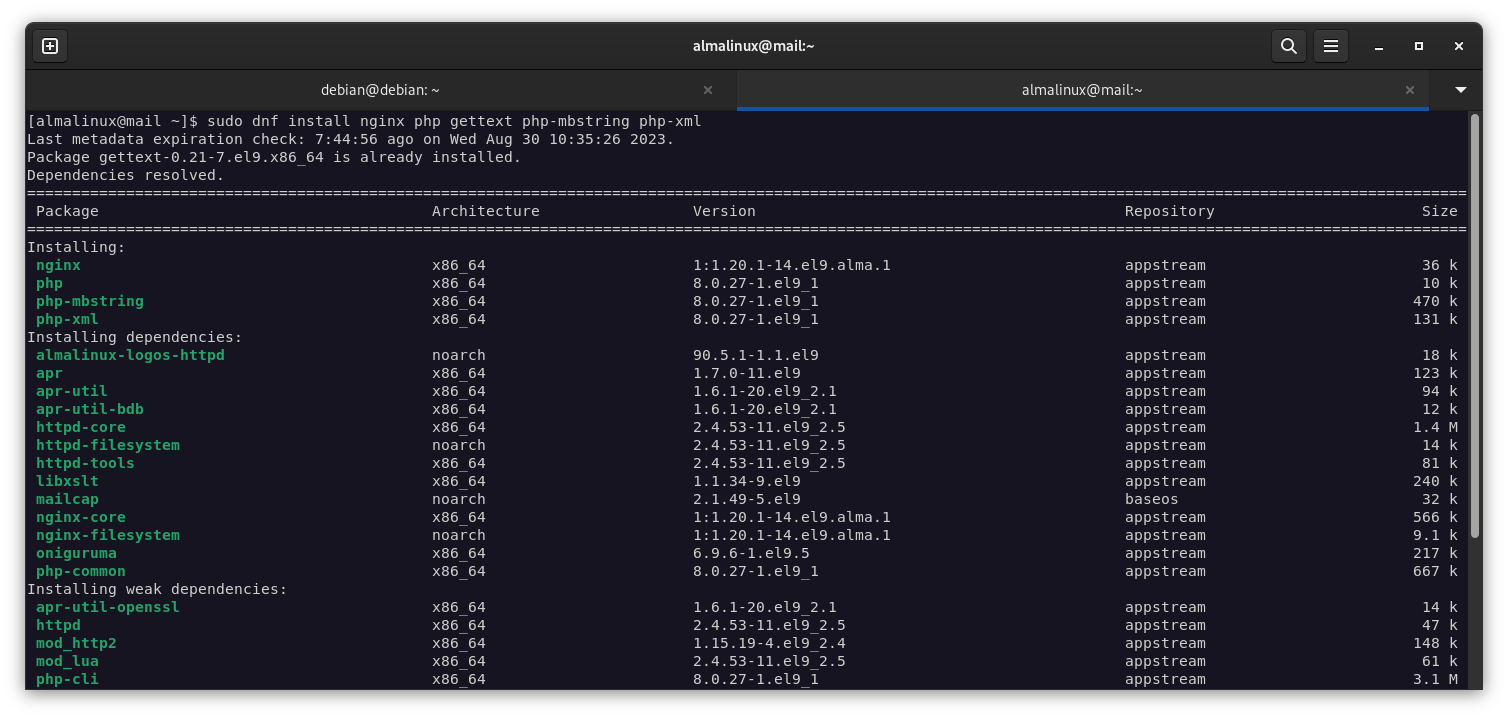
\includegraphics[scale=0.30]{21}
	\caption{Instalación del servicio web.}
\end{figure}

Ahora configuramos la ruta de la carpeta junto al nombre de dominio que va a tener el servicio web. Dicho nombre de dominio es el mismo que va a tener el servidor de correo.

\begin{figure}[H]
	\centering
	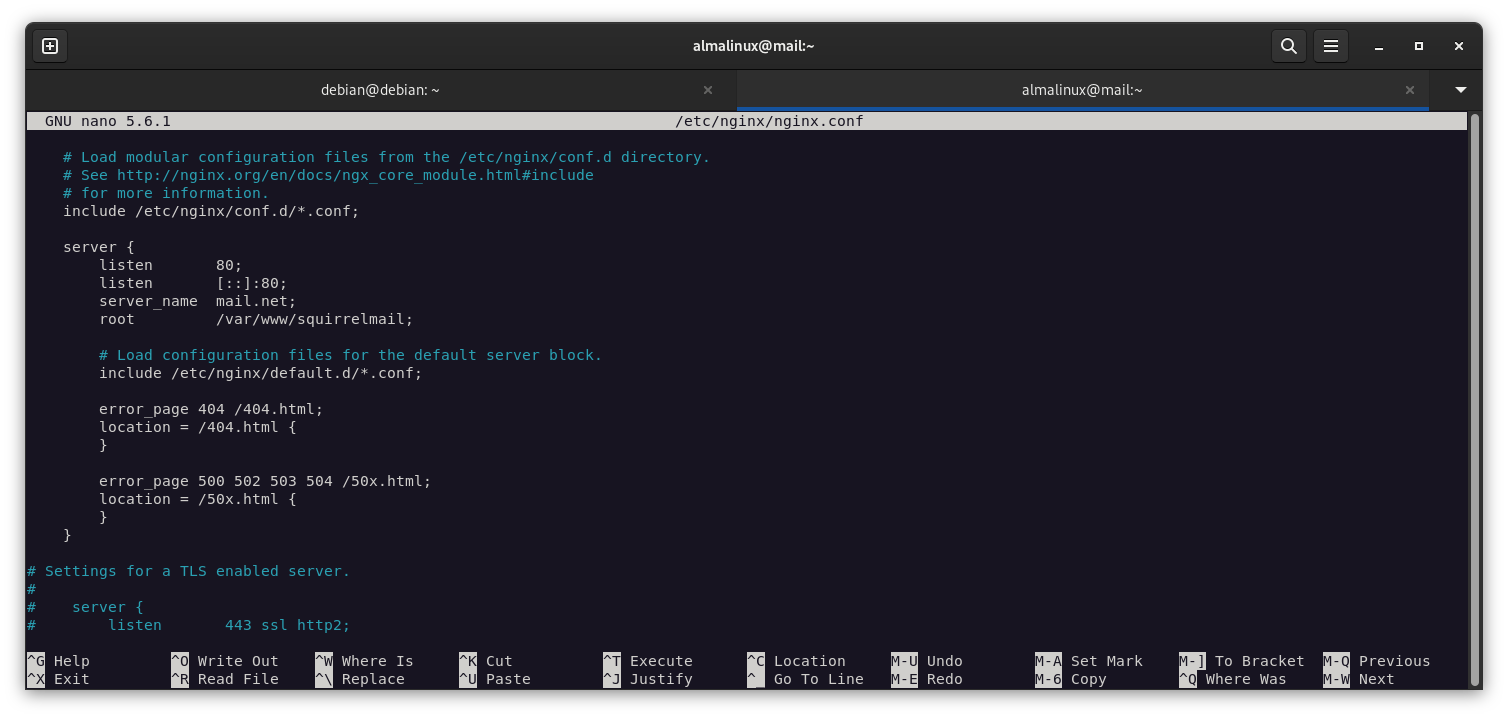
\includegraphics[scale=0.30]{22}
	\caption{Configuración de NGINX.}
\end{figure}

Ahora para configurar squirrelmail, aparte de descargarnos los ficheros desde su web, tenemos que instalar perl, porque tiene un script que te ayuda a crear el fichero de configuración que necesita el servicio.

\begin{figure}[H]
	\centering
	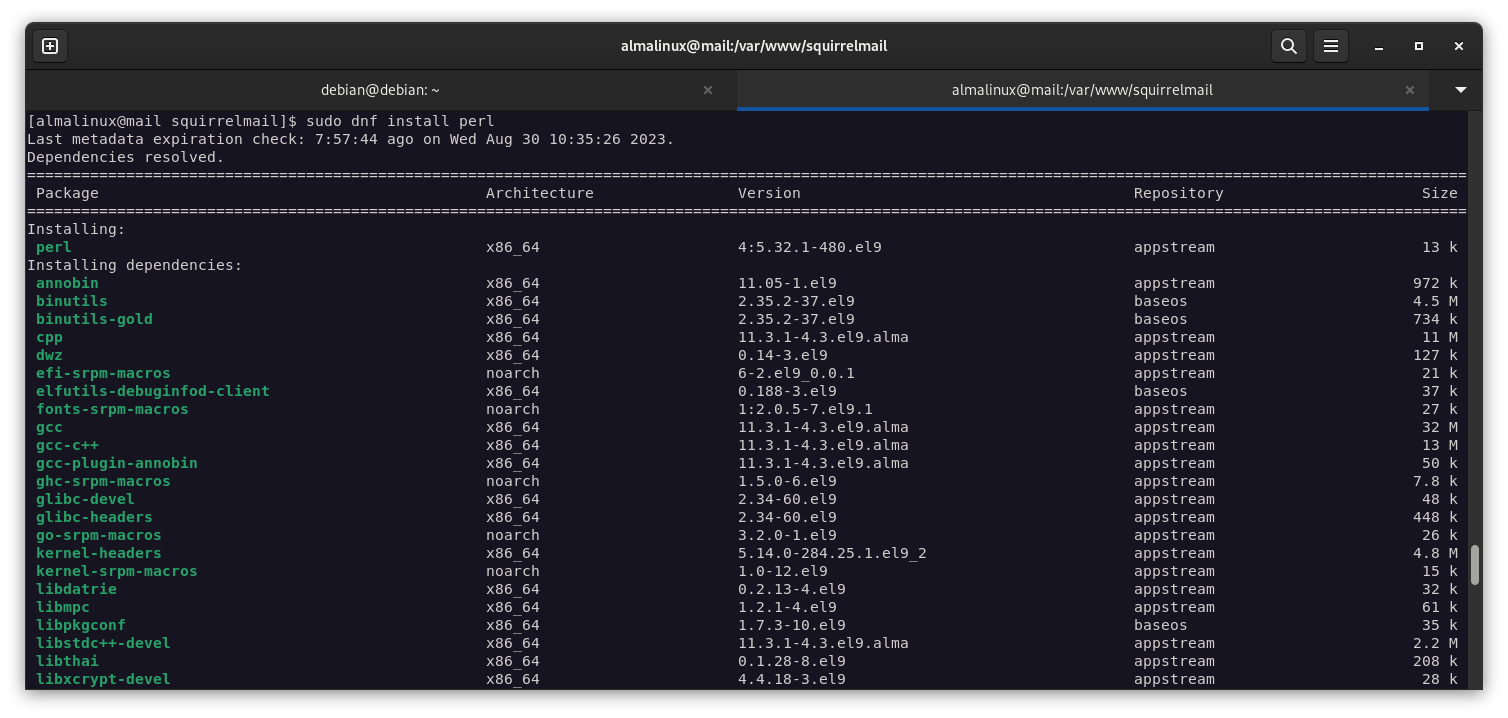
\includegraphics[scale=0.30]{23}
	\caption{Instalación de perl.}
\end{figure}

\begin{lstlisting}[style=mybash]
sudo dnf install perl
# Luego de instalar, en /var/www/squirrelmail
sudo perl config/conf.pl
\end{lstlisting}

Ahora lanzamos el menú de configuración.

\begin{figure}[H]
	\centering
	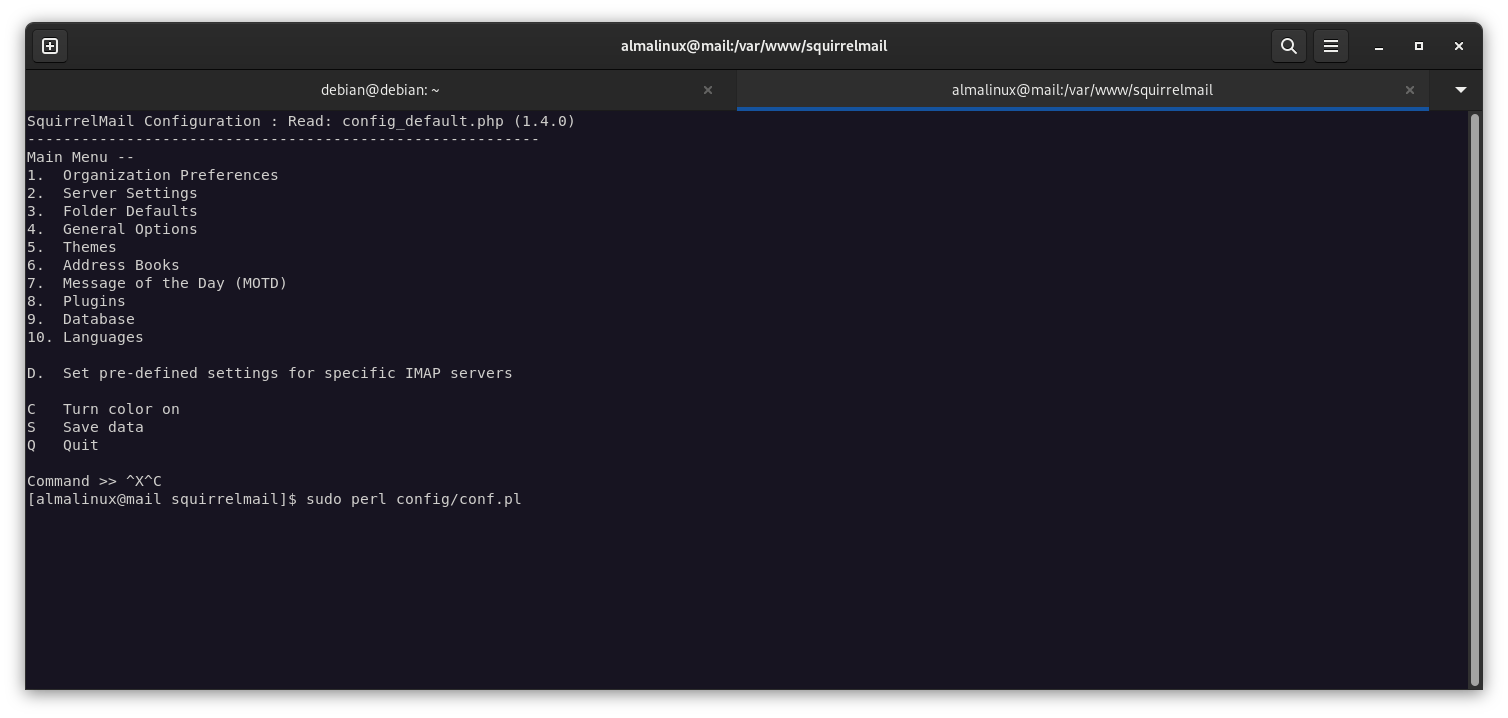
\includegraphics[scale=0.30]{24}
	\caption{Configurador de squirrelmail.}
\end{figure}

Nos vamos a la opción 2 para configurar el servidor web. Cambiamos el nombre de dominio y el resto lo dejamos en localhost.

\begin{figure}[H]
	\centering
	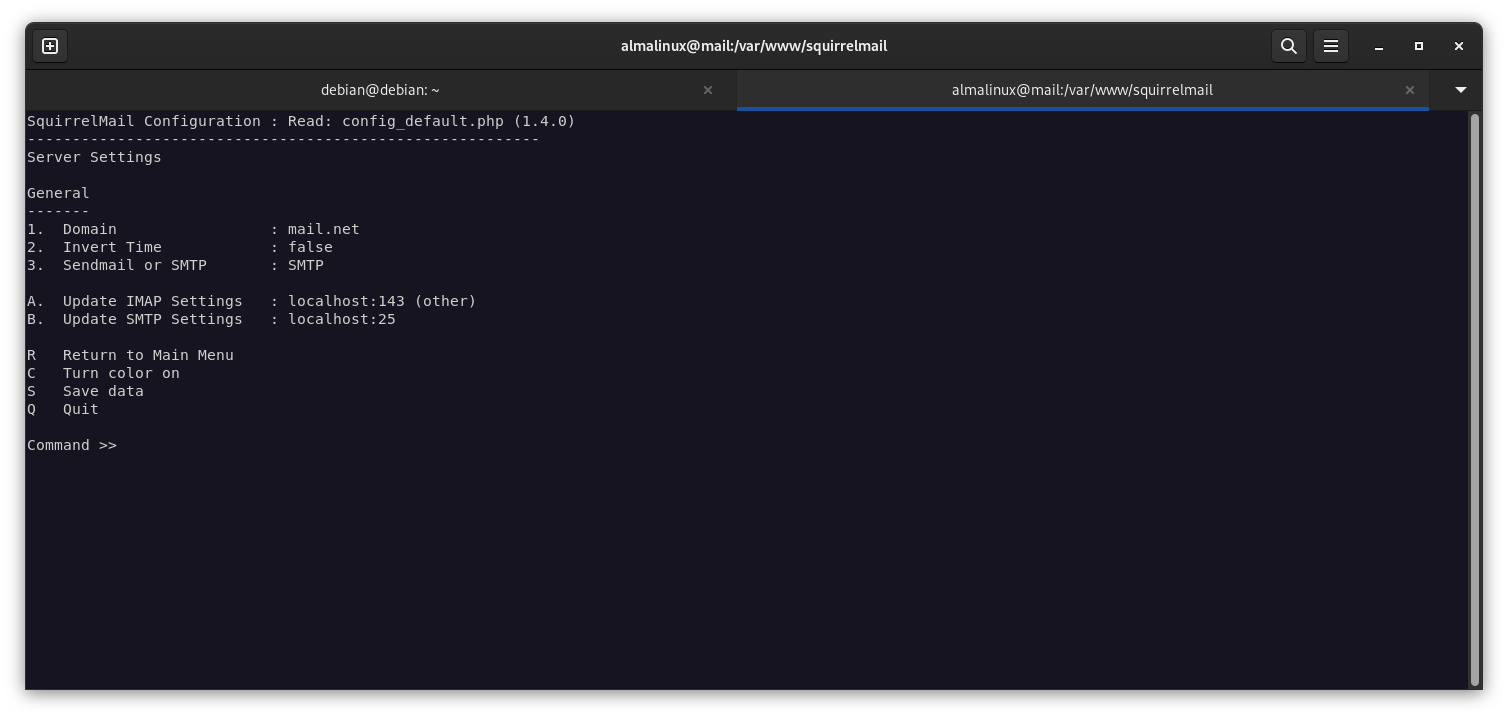
\includegraphics[scale=0.30]{25}
	\caption{Configurador de squirrelmail - Opción 2.}
\end{figure}

Finalmente ejecutamos los siguientes comandos al terminar de ejecutar el script configurador, esto es necesario para generar el correcto funcionamiento del servicio web que necesita unos directorios especiales.

\begin{lstlisting}[style=mybash]
# Necesita que las carpetas las tenga el mismo usuario que el servicio web
sudo chown -R nginx:nginx /var/www/squirrelmail/
sudo mkdir -p /var/local/squirrelmail/data
sudo chown -R nginx:nginx /var/local/squirrelmail/
# Esto es neceario para permitir la conectividad con IMAP
sudo setsebool httpd_can_network_connect=1
\end{lstlisting}

\begin{figure}[H]
	\centering
	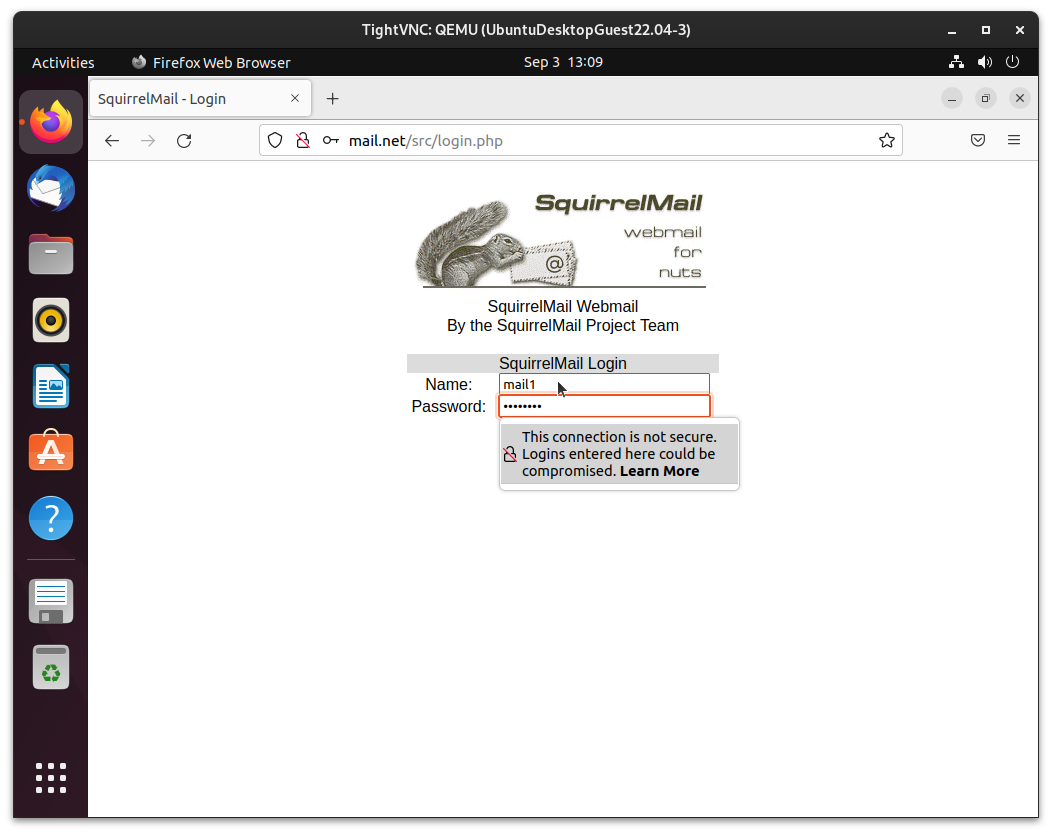
\includegraphics[scale=0.30]{27}
	\caption{Servicio web activado.}
\end{figure}

\begin{figure}[H]
	\centering
	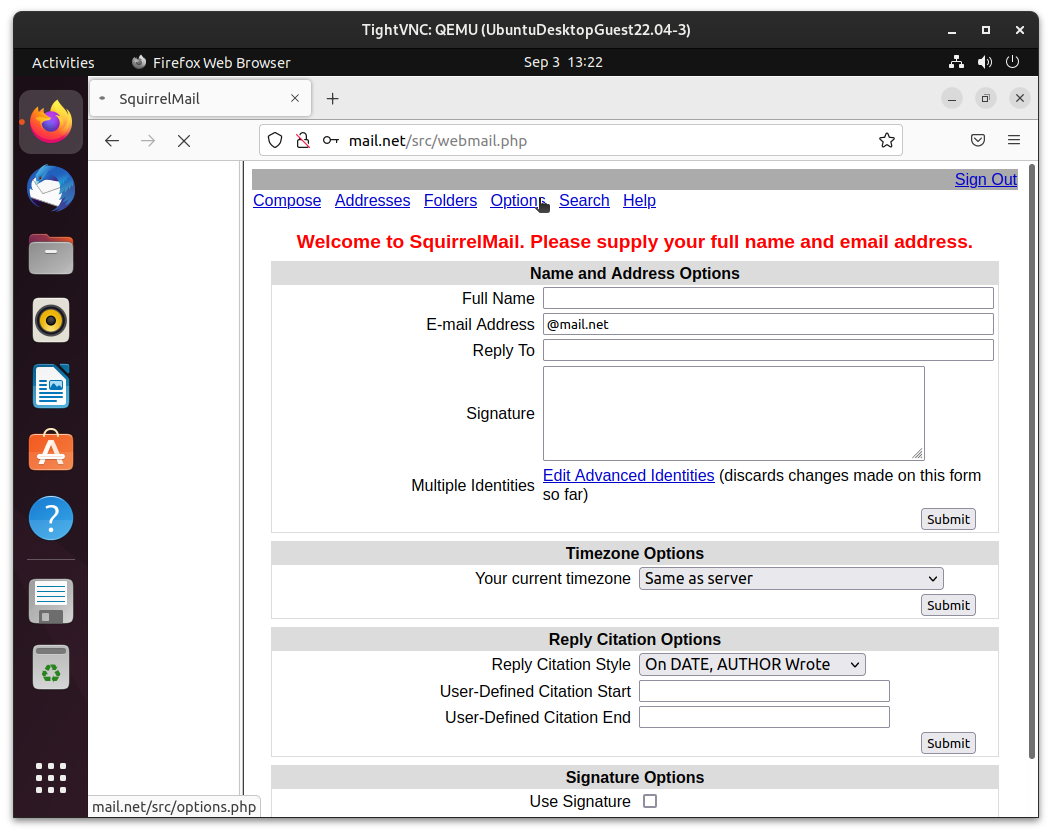
\includegraphics[scale=0.30]{28}
	\caption{Servicio web activado - Parte 2.}
\end{figure}

Notas: Debido a la versión de PHP, algunas funciones no funcionan como deben debido a lo obsoleto del software, por lo que se ha modificado el siguiente archivo la parte del if (donde se ha quitado un !), para que pueda funcionar y verse el menú. Pero sigue teniendo un estado erróneo. En concreto no te deja autenticarte como usuario, quedándose en un bucle donde no puedes salir del menú de autenticación.

\begin{figure}[H]
	\centering
	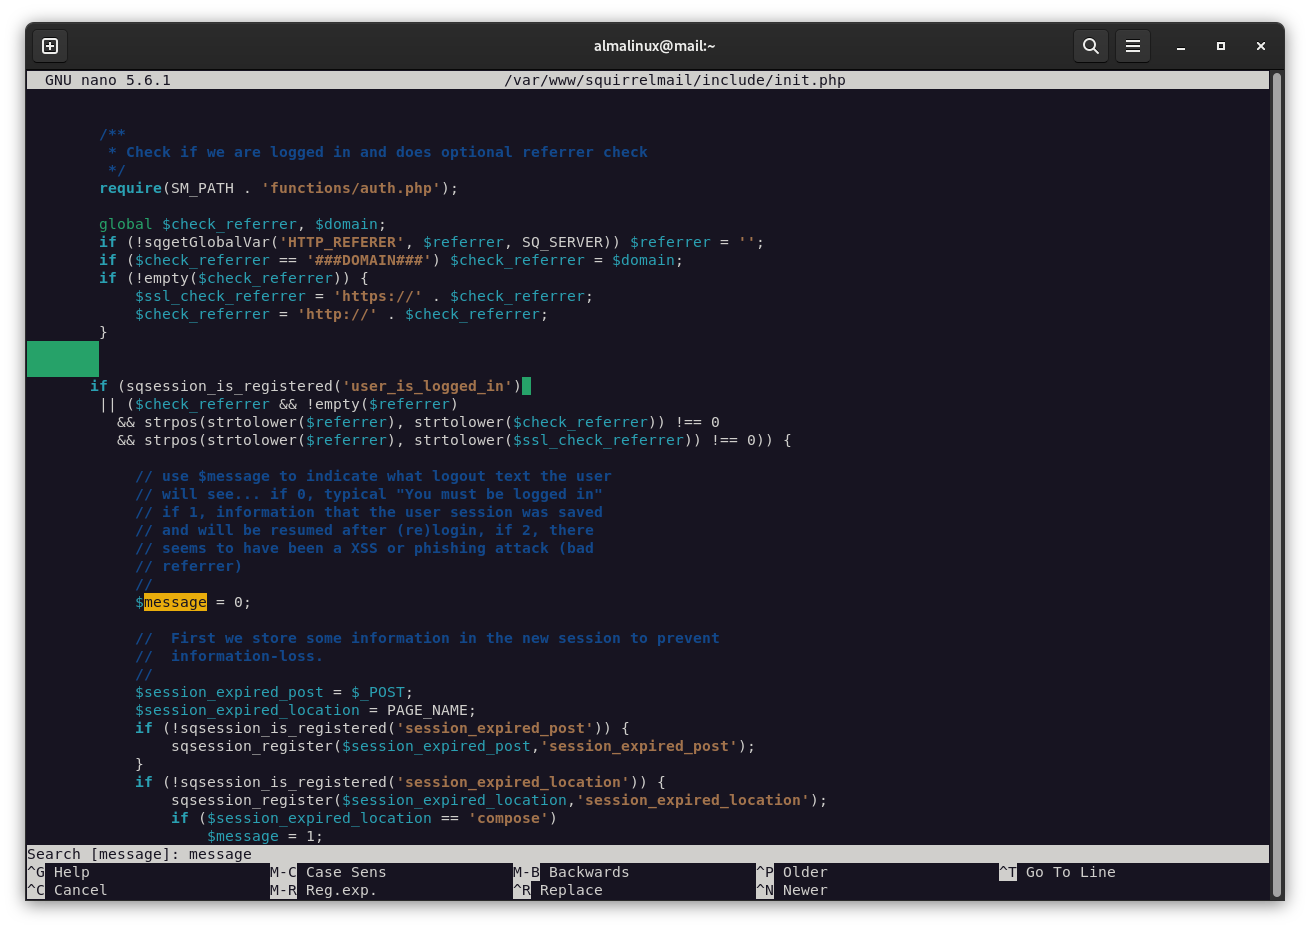
\includegraphics[scale=0.30]{29}
	\caption{Parte que da error.}
\end{figure}

%\begin{figure}[H]
%	\centering
%	\includegraphics[scale=0.30]{cuestion_1_1}
%	\caption{Se puede ver que al no haber un fallo grave, el sistema lo nota como que sigue funcionando pero en un estado degradado.}
%\end{figure}

%\newpage

%Se pueden hacer include en latex
%\newpage

\section{Section}

\subsection{Subseccion}

\subsubsection{Subseccion}



%-------Bibliografia-----------------------------

%\newpage
\section{Bibliografía}

% Ejemplo
\footnote{Administración de mdadm - Por Red Hat}
\textcolor{blue}{\url{https://access.redhat.com/documentation/en-us/red_hat_enterprise_linux/8/html/managing_storage_devices/managing-raid_managing-storage-devices#monitoring-raid_managing-raid}}



\end{document}
